\documentclass{beamer}
\usetheme{metropolis} % Use metropolis theme





\title{ECON 3818: Introduction to Statistics with Computer Applications}
%\subtitle
\date{\today}
\author{Kyle Butts}



\definecolor{blue}{RGB}{0,114,178}

\definecolor{red}{HTML}{EB0E09}
\definecolor{yellow}{RGB}{240,228,66}
\definecolor{green}{RGB}{0,158,115}
\definecolor{maroon}{HTML}{AF3335}
\definecolor{purple}{HTML}{7E90B8}


\definecolor{mybackground}{HTML}{ECECEC}
\setbeamercolor{background canvas}{bg= mybackground}

\definecolor{buff-gold}{HTML}{CFB87C}
\definecolor{buff-grey}{HTML}{565A5C}
\definecolor{buff-lightgrey}{HTML}{A2A4A3}
\definecolor{buff-black}{HTML}{000000}

\setbeamercolor{alerted text}{fg=buff-gold!80!black}
\setbeamercolor{frametitle}{bg=buff-black}
\setbeamercolor{title}{fg=buff-grey}
\setbeamercolor{button}{bg=buff-gold}

% Allow to remove indent w/ \begin{itemize}[leftmargin= *]
\usepackage{enumitem}
\setlist[itemize]{label= \textbullet}

% \usepackage[libertine]{newtxmath}
\usepackage{longtable}
\usepackage{booktabs}
\usepackage{enumitem}







\begin{document}

% Title Page ---------------------------------------
\maketitle


% Introduction -------------------------------------
\section{Introduction}
\begin{frame}{What to expect from the course}
	
	\begin{itemize}
		\item Objectives: 
            \begin{itemize}
		      	\item Give you a background on statistical theory and their application
		      	\item Learn how to perform basic statistical analysis in the R programming language
		      	\item Prepare you to succeed in econometrics courses  
            \end{itemize}
	\end{itemize}
\end{frame}


\begin{frame}{Grading Summary}
    \begin{center}
        \small{
            \begin{tabular}{| l | c |}
                \hline
                \textbf{Assignment} & \textbf{Percentage}\\ 
                \hline
                Homework & 10\% \\ \hline
                R Problem Sets & 10\% \\ \hline 
                R Project & 10\% \\ \hline 
                Midterm 1 & 20\% \\ \hline
                Midterm 2 & 20\%  \\ \hline
                Final & 20\%  \\ \hline
            \end{tabular}}
    \end{center}
\end{frame}


\begin{frame}{Expectations for Students}
	
	\begin{itemize}
		\item Homework \& R Homework
            \begin{itemize}
		      	\item Weekly homeworks are assigned, the best way to learn mathematics is \textbf{practice, practice, practice}
		      	\item Absolutely NO late homework; will drop the lowest two homeworks and the lowest R homework.
            \end{itemize}

		\item Attendance
            \begin{itemize}
		      	\item Really important to attend lecture to get handle on new material, but no attendance will be taken.
		      	\item Clicker questions will count for extra credit
            \end{itemize}

        \item Recitation
            \begin{itemize}
                \item Recitation attendance is not mandatory, but if you are going to study for 1 hour/week, recitation is the best place to do it. You will walk through examples and really helpful for prepping for exams
            \end{itemize}
	\end{itemize}
	
\end{frame}

\begin{frame}{Expectations for Students}
	
	\begin{itemize}
        \item R Project
            \begin{itemize}
                \item You will download real world data and perform basic statistical analysis and create data visualizations.
            \end{itemize} 

		\item Midterm \& Final Exam
            \begin{itemize}
		      	\item NO makeup midterms, weight of missed midterm will be added to final
		      	\item Must inform me of any accommodations \textbf{two weeks} before an exam
            \end{itemize}
	\end{itemize}
	
\end{frame}

\begin{frame}{Coronavirus}
    \begin{itemize}
        \item If you have the coronavirus and are asymptomatic, just attend lecture remotely and continue through the course.
        \item If you have the coronavirus and are sick, email me so we can make plans to keep you on track in the course. Communication is \textbf{key}.
    \end{itemize}
\end{frame}


\begin{frame}{What is Statistics?}
	
	\begin{itemize}
		\item Statistics gives us a way of linking economic theory with the real world through data analysis
		      \begin{itemize}
		      	\item How did the market react when interest rates went up? 
		      	\item How did firms respond to a new government policy?
		      \end{itemize}

		\item Statistics allows us to translate datasets into usable information
		      \begin{itemize}
		      	\item Summary statistics help describe large groups of data
		      	\item Use statistics to make predictions
		      	\item Statistics helps us inform our decision making
		      \end{itemize}
	\end{itemize}
	
\end{frame}


\begin{frame}{Real-world examples - Coronavirus Tracking}
    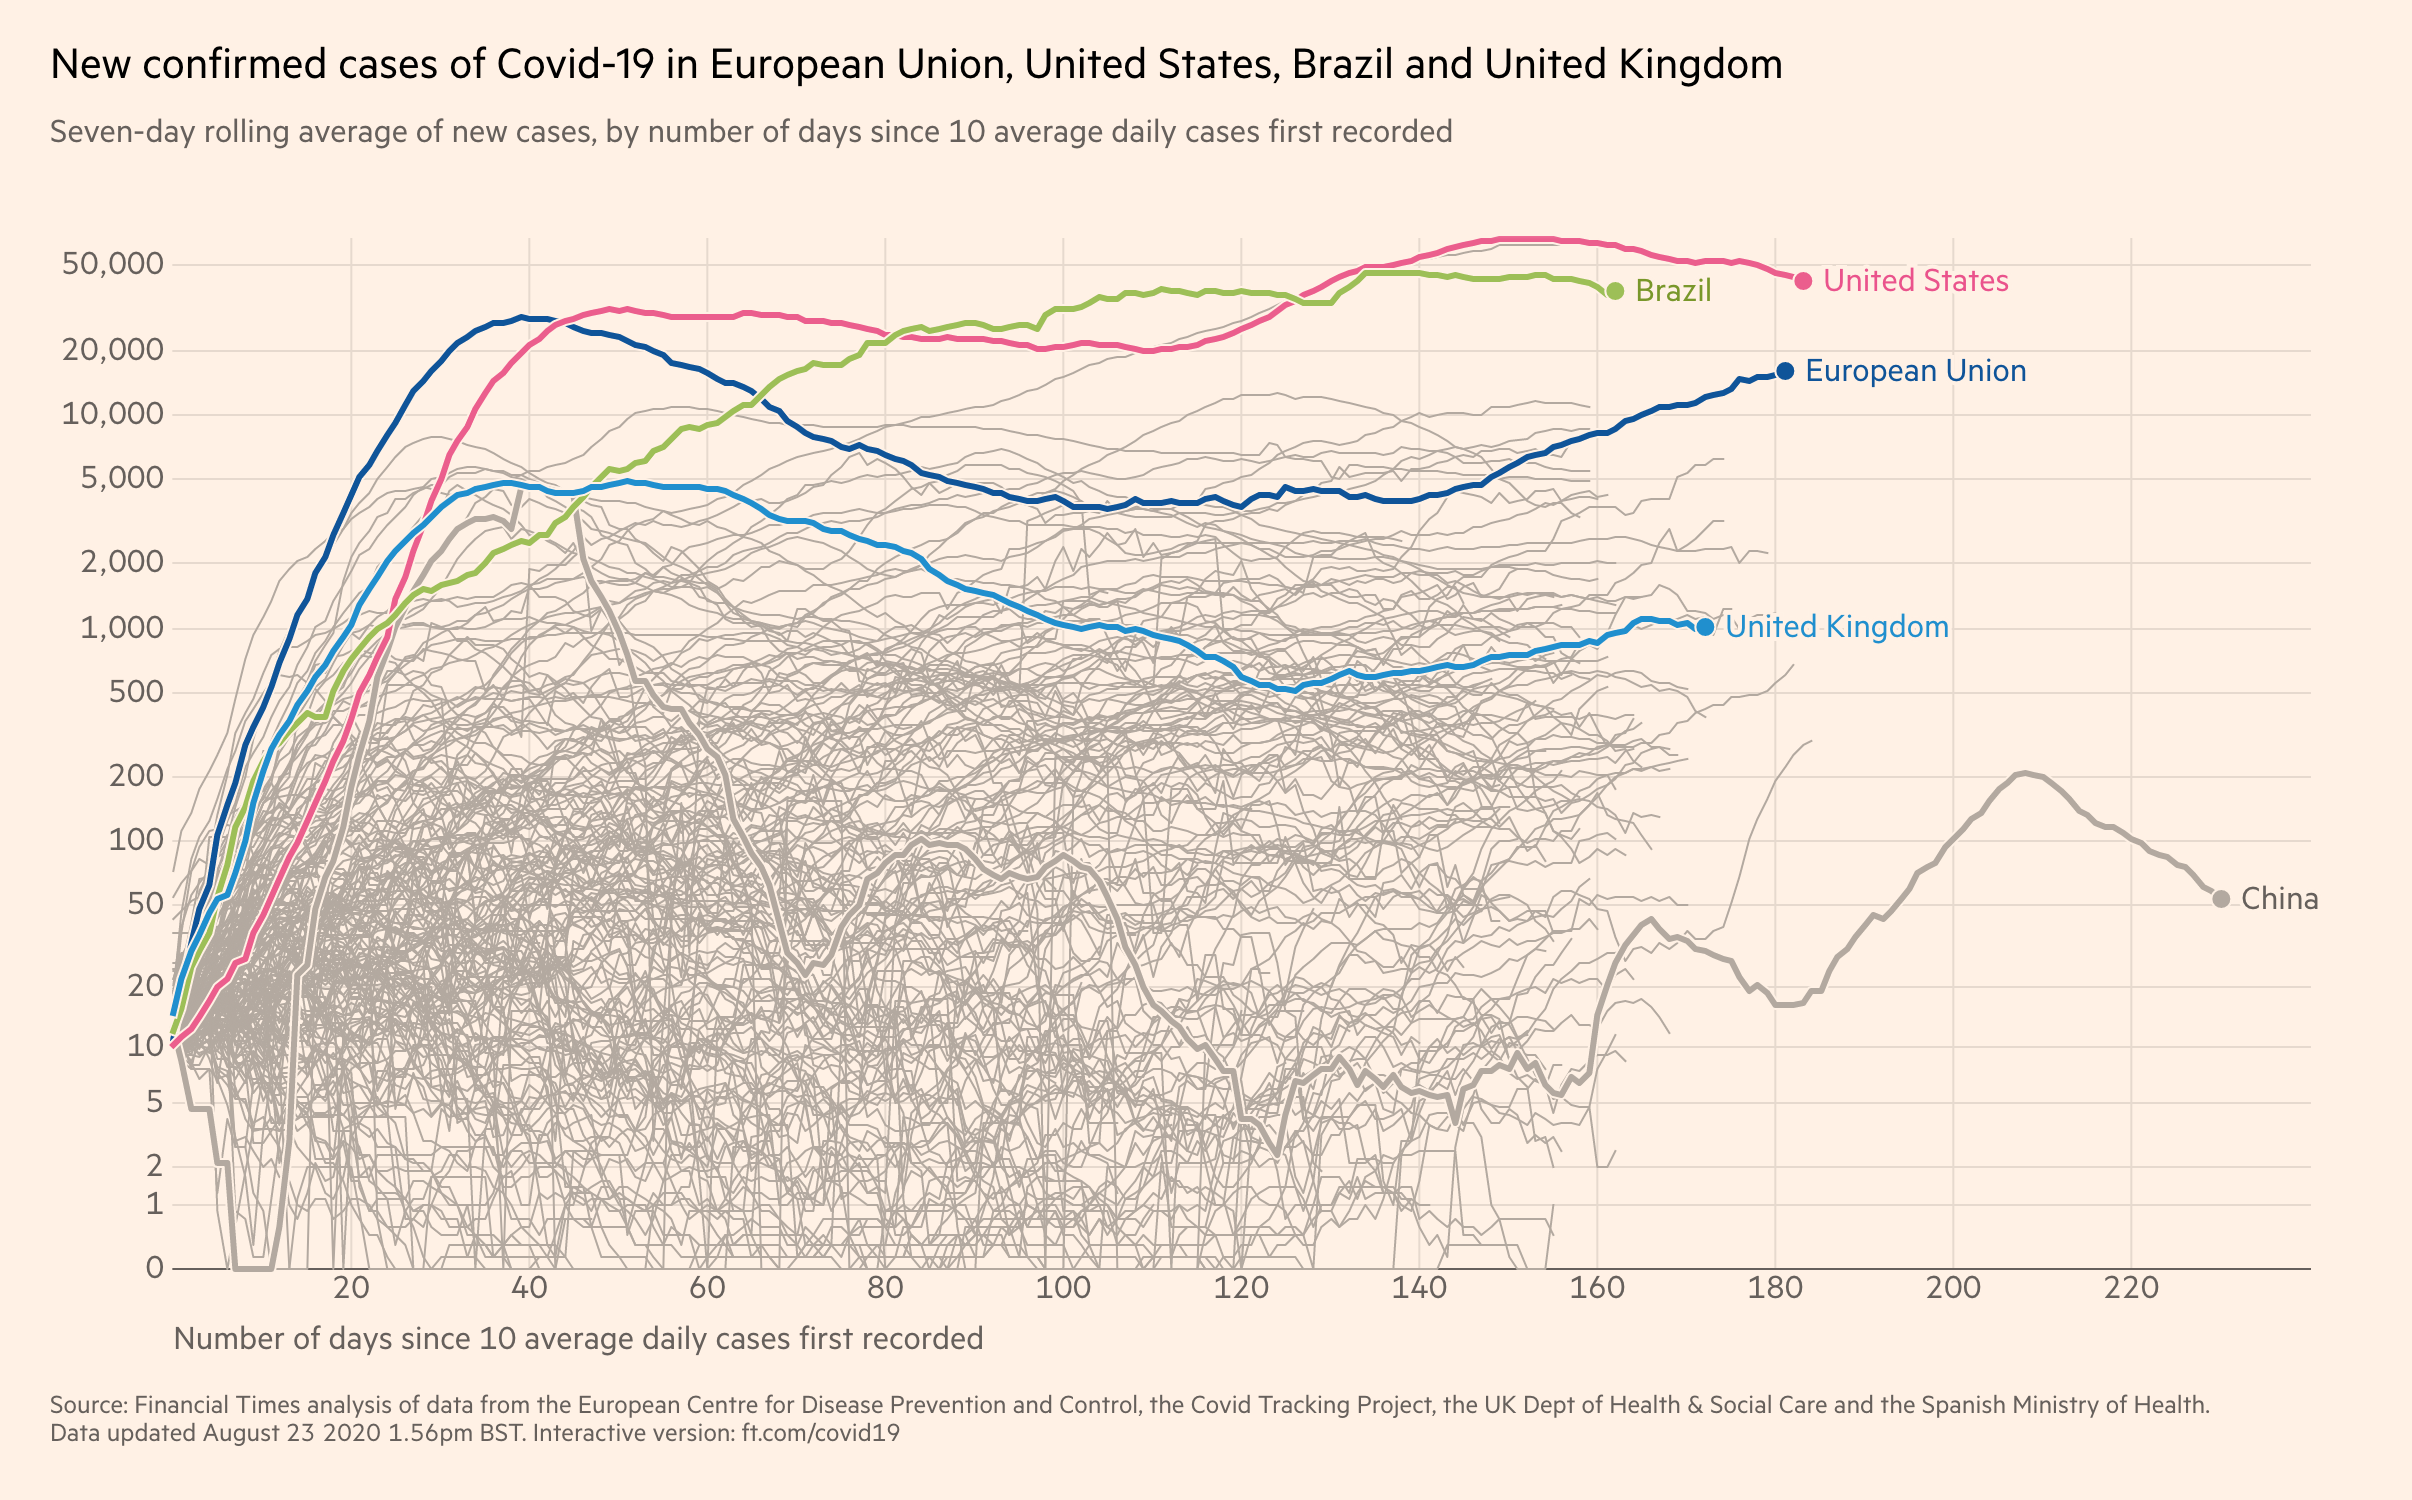
\includegraphics[width=\linewidth]{coronavirus.png}
\end{frame}


\begin{frame}{Real-world examples - Weather Prediction}
    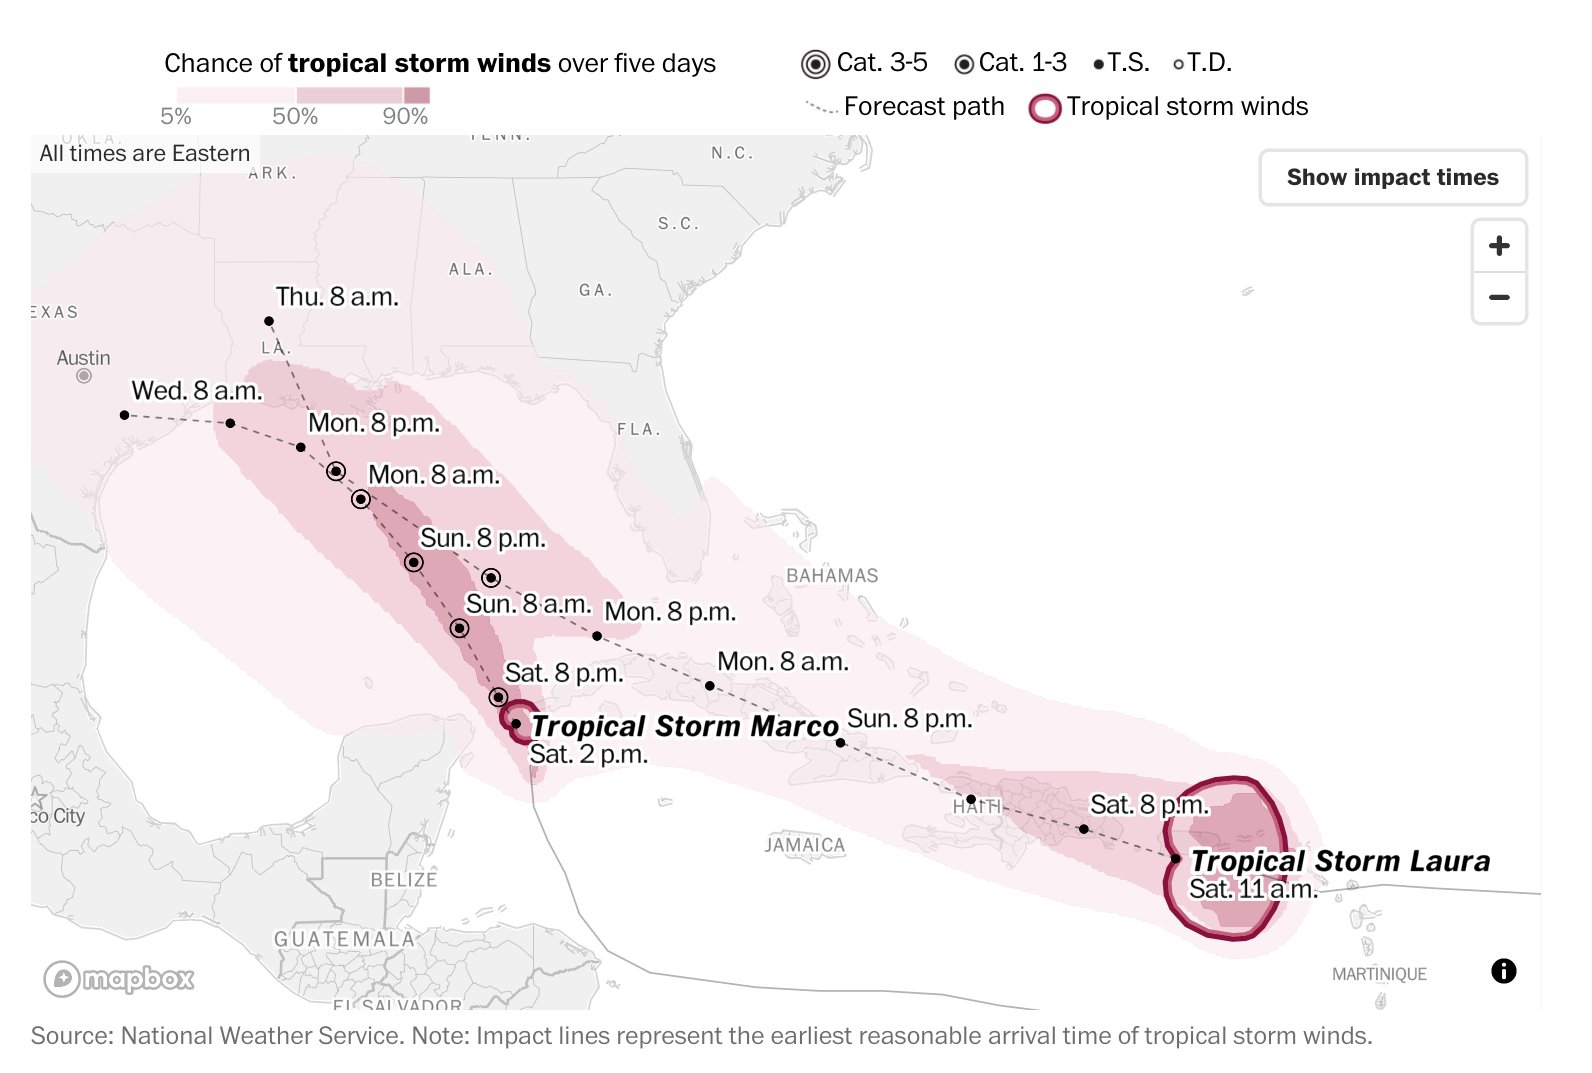
\includegraphics[width=\linewidth]{hurricane.jpg}
\end{frame}

\begin{frame}{Real-world examples - Climate Change}
    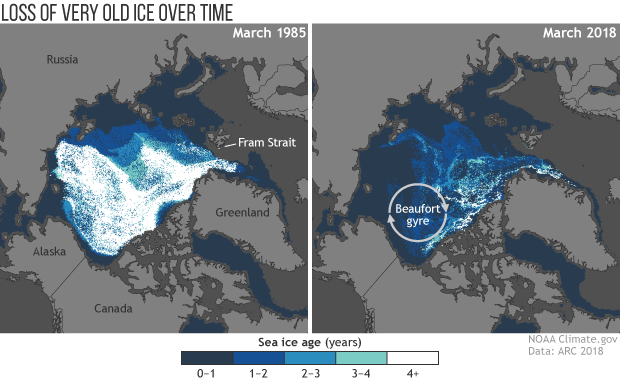
\includegraphics[width=\linewidth]{sea_ice.png}
\end{frame}

\begin{frame}{Real-world examples - Election Predictions}
    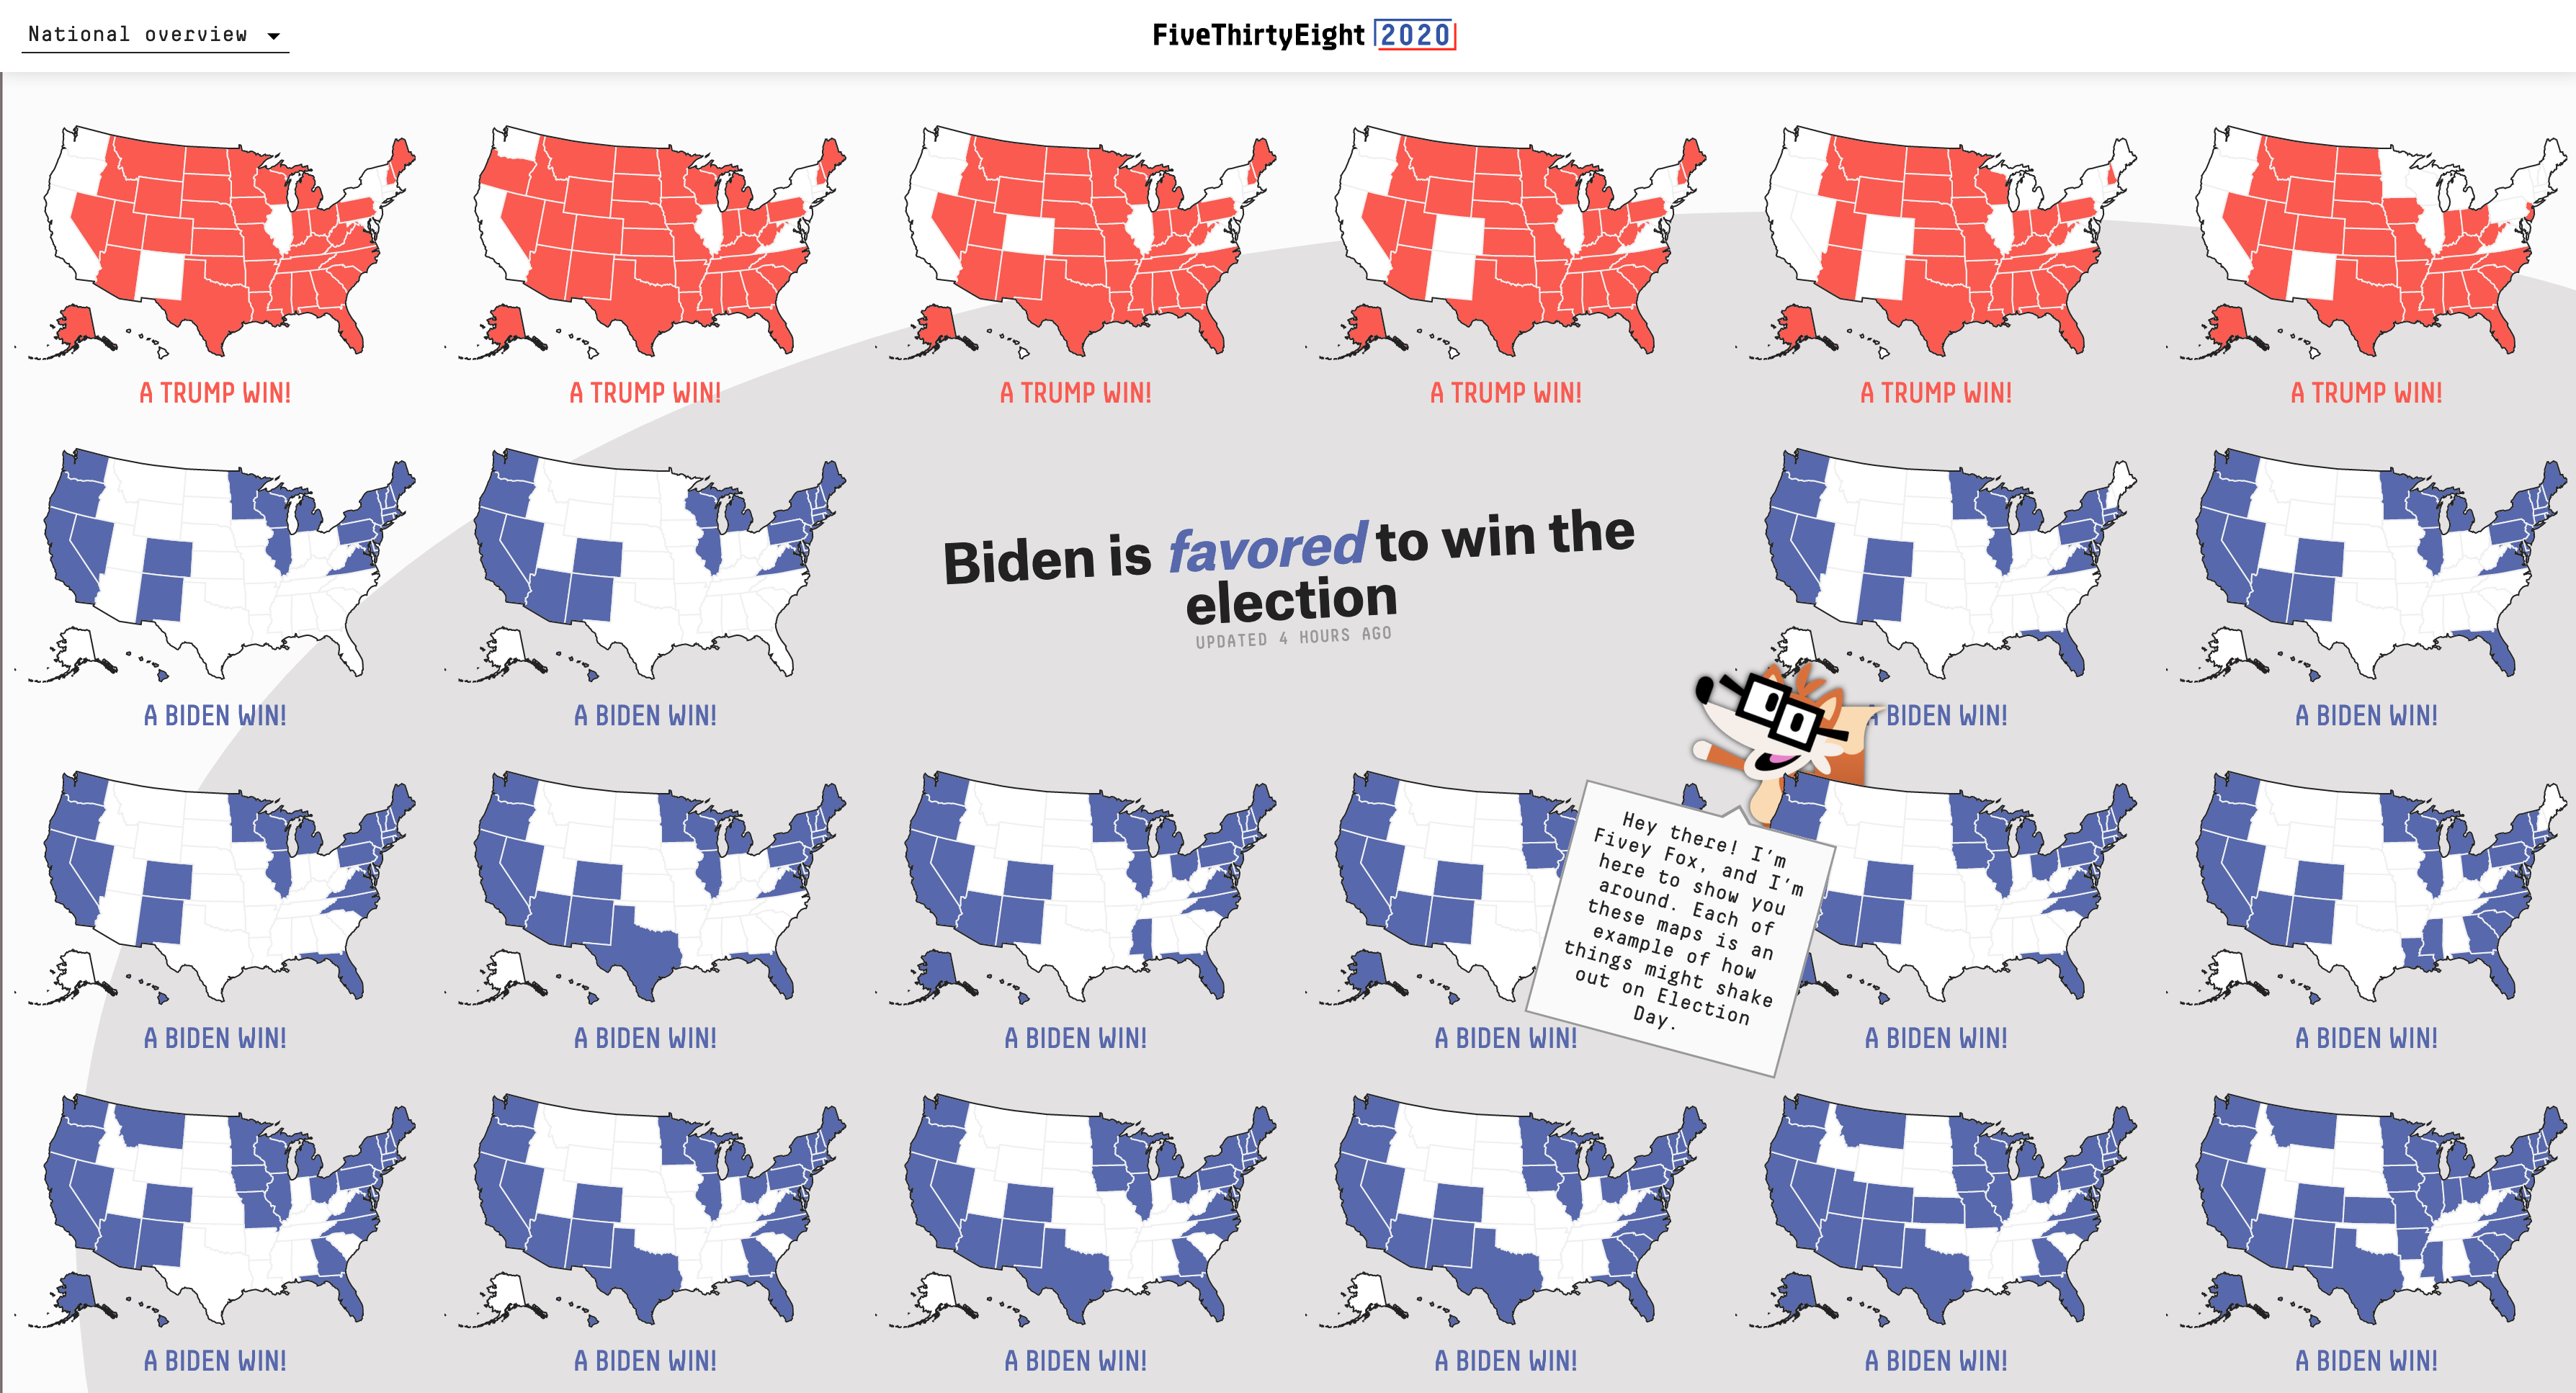
\includegraphics[width=\linewidth]{538_1.png}
\end{frame}

\begin{frame}{Real-world examples - Election Predictions}
    \begin{center}
        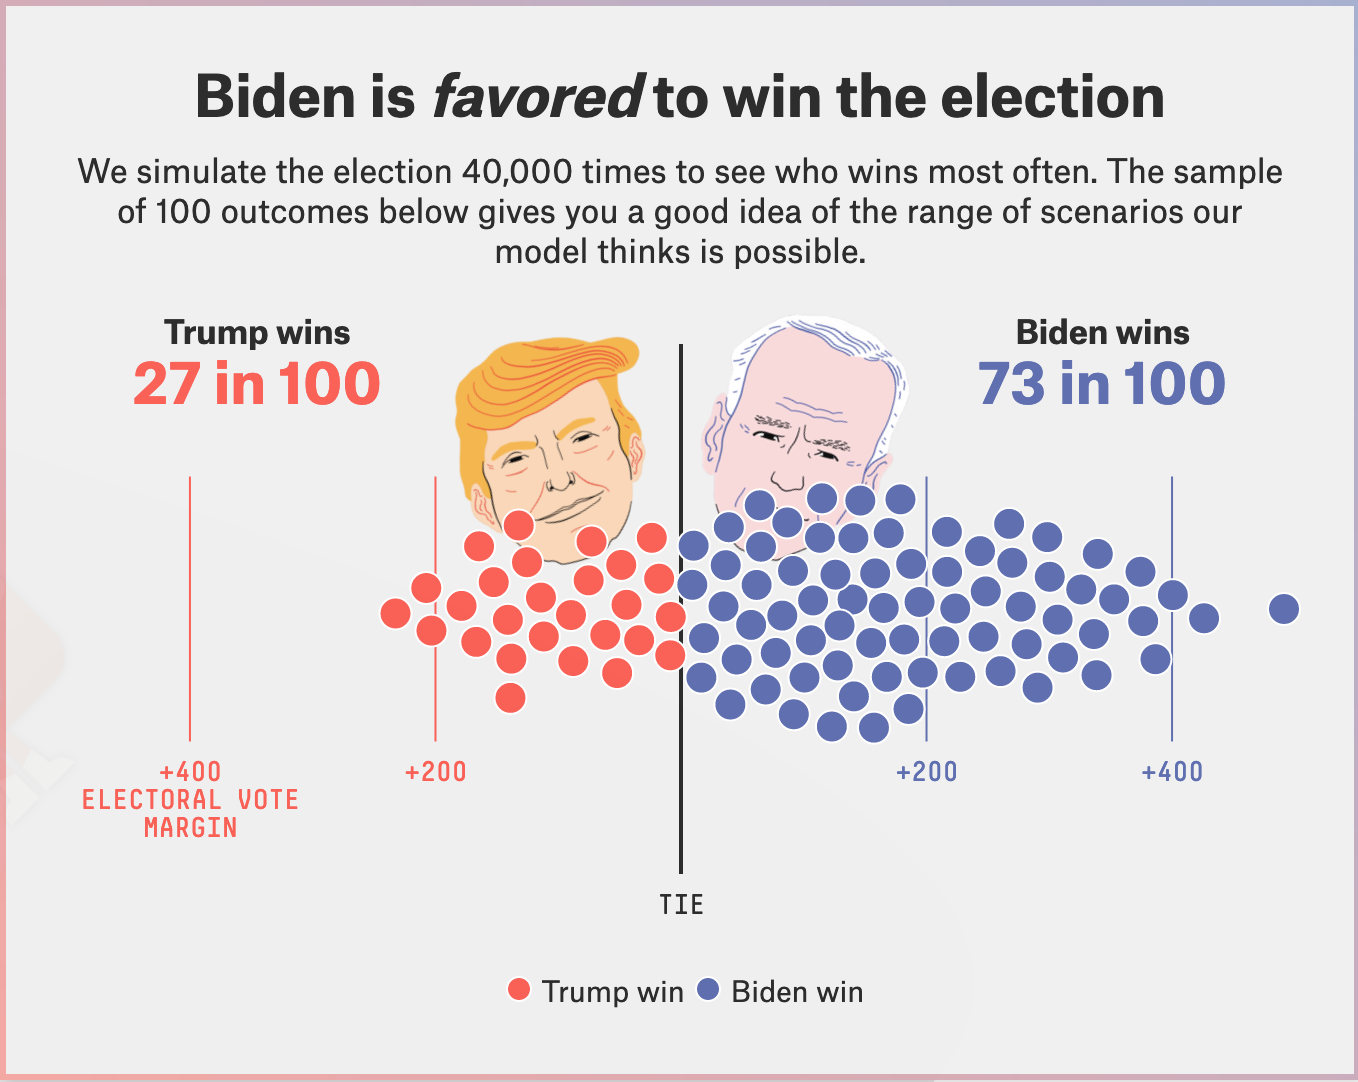
\includegraphics[width=0.9\linewidth]{538_2.png}
    \end{center}
\end{frame}

\begin{frame}{Real-world examples - Election Predictions}
    \begin{center}
        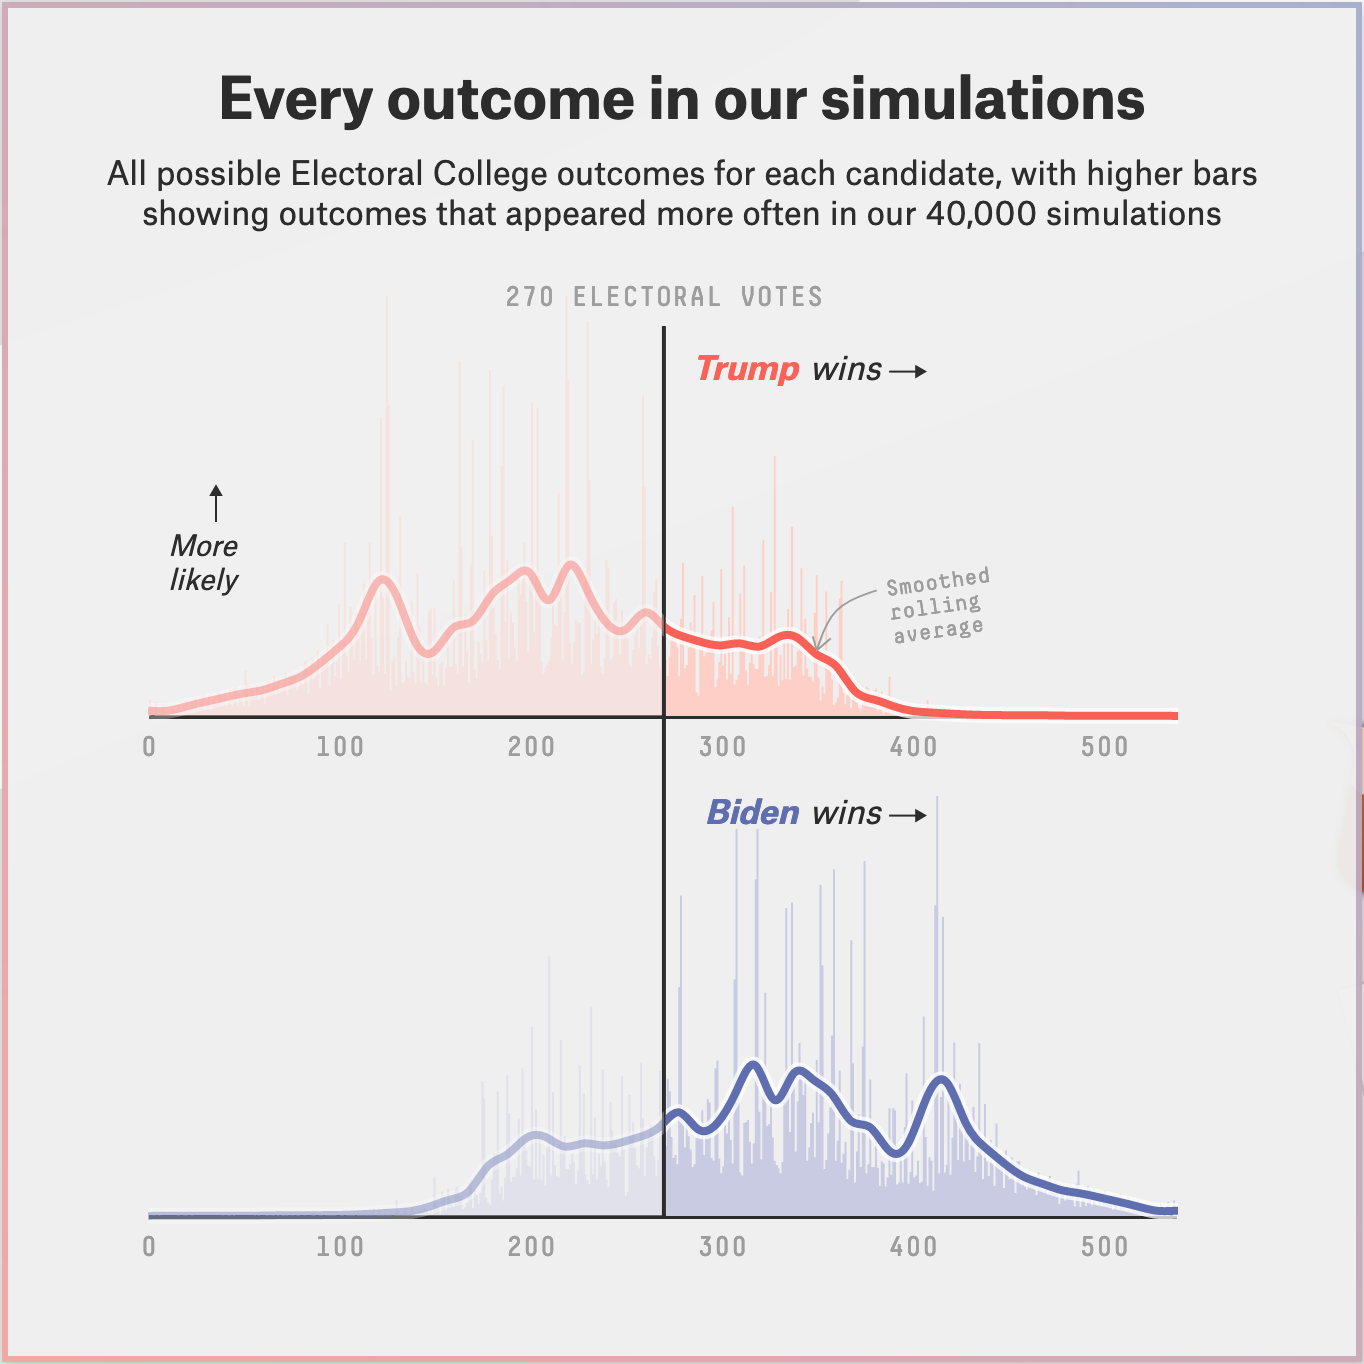
\includegraphics[width=0.75\linewidth]{538_3.png}
    \end{center}
\end{frame}

\begin{frame}{Other uses of Statistics}
	
	Statistics is used in a variety of different ways/fields
	\begin{itemize}
		\item Financial markets
		\item Science/medical research
		\item Purchasing insurance --- how risky are you to insure?
		\item Sports -- think Moneyball
	\end{itemize}
	
\end{frame}






% Chapter 1 ----------------------------------------
\section{Chapter 1: Picturing Distributions with Graphs}

\begin{frame}{Statistics}
    \begin{itemize}
        \item \alert{Statistics}: the science of data. Deals with the collection, organization, analysis, interpretation and presentation of data
        \item Use statistics to identify patterns and trends in the data in order to inform decision-making
    \end{itemize}
\end{frame}

\begin{frame}{Observations and Variables}
    \begin{itemize}
        \item \alert{Observation}: an individual unit of analysis in the dataset
        \begin{itemize}
            \item Examples: person, state, country, etc.
        \end{itemize}
        
        \item \alert{Variable}: characteristic of an observation
        \begin{itemize}
            \item Examples: age, population, GDP, etc.
        \end{itemize}
    \end{itemize}

    \begin{center}
    \scalebox{0.7}{
        \begin{tabular}{| c | c | c | c | c |}
        \hline
        \textbf{Player Name} & \textbf{Position} & \textbf{Team}  & \textbf{Salary} & \textbf{Contract Length} \\ [0.25ex]
        \hline
        Stephen Curry & Point Guard & Golden State Warriors & \$40.2 million & 5 years \\
        \hline
        Russell Westbrook & Point Guard & Houston Rockets & \$38.5 million & 5 years \\
        \hline
        Chris Paul & Point Guard & Oklahoma City Thunder & \$38.5 million & 4 years \\
        \hline
        Lebron James & Small Forward & Los Angeles Lakers & \$37.4 million & 4 years \\ 
        \hline
        James Harden & Shooting Guard & Houston Rockers & \$38.2 million & 4 years \\
        \hline
        Kevin Durant & Small Forward & Brooklyn Nets & 37.2 million & 4 years \\
        \hline
        \end{tabular}
    }
    \tiny{Data provided by Business Insider}
    \end{center}

\end{frame}

\begin{frame}{Type of Variables}
    \begin{itemize}
        \item \alert{Categorical variable}: takes on a unique value for each possible category or trait
            \begin{itemize}
                \item Examples: race, political party, dog breed, etc.
            \end{itemize}
        \item \alert{Quantitative variable}: measured on a numeric scale
            \begin{itemize}
                \item income, unemployment rate, weight, etc.
            \end{itemize}
        \item Variables may be either \alert{discrete} (countable) or \alert{continuous} (uncountable)
    \end{itemize}

    \begin{center}
        \scalebox{0.7}{
            \begin{tabular}{| c | c | c | c | c |}
            \hline
            \textbf{Player Name} & \textbf{Position} & \textbf{Team}  & \textbf{Salary} & \textbf{Contract Length} \\ [0.25ex]
            \hline
            Stephen Curry & Point Guard & Golden State Warriors & \$40.2 million & 5 years \\
            \hline
            Russell Westbrook & Point Guard & Houston Rockets & \$38.5 million & 5 years \\
            \hline
            Chris Paul & Point Guard & Oklahoma City Thunder & \$38.5 million & 4 years \\
            \hline
            Lebron James & Small Forward & Los Angeles Lakers & \$37.4 million & 4 years \\ 
            \hline
            James Harden & Shooting Guard & Houston Rockers & \$38.2 million & 4 years \\
            \hline
            Kevin Durant & Small Forward & Brooklyn Nets & 37.2 million & 4 years \\
            \hline
            \end{tabular}
        }
        \tiny{Data provided by Business Insider}
    \end{center}
\end{frame}

\begin{frame}{Clicker Question}
    Given the following dataset, which of these statements is correct?
    
    \begin{center}
    \scalebox{0.7}{
    \begin{tabular}{|l | r | r | l | r |}
        \toprule
        % Head -----------------------------------------
        \textbf{State} & \textbf{Year} & \textbf{Electricity Sales} & \textbf{Government} & \textbf{Renewable Capacity} \\ 
        \midrule

        % Body -----------------------------------------
        AK & 2000 & 5249376 & D & 0 \\ \hline
        AL & 2000 & 77469092 & D & 493 \\ \hline
        AR & 2000 & 35596936 & R & 369 \\ \hline
        AZ & 2000 & 63545095 & R & 1 \\ \hline
        CA & 2000 & 219633132 & D & 3053 \\ \hline
        CO & 2000 & 46563544 & R & 29 \\ \hline
        CT & 2000 & 33605197 & R & 262 \\
        \bottomrule
    \end{tabular}
    }
    \end{center}

    \begin{enumerate}[label=(\alph*)]
        \item Electricity sales, renewable capacity and state are all quantitative variables
        \item Government, state are both categorical variables
        \item All variables are categorical
        \item All variables are quantitative
    \end{enumerate}
\end{frame}

\begin{frame}{Categorical Variables as Dummy Variables}
    Often time in datasets, \alert{dummy variables}, or indicator variables, are used to describe categorical variables. 

    \begin{itemize}
        \item For example, we could define the "Government" variable as 0 for D and 1 for R. 
        \item Dummy/indicator variables put observations into categories, even though they are numerical in value
    \end{itemize}
\end{frame}

\begin{frame}{Distribution of a Variable}
    \begin{itemize}
        \item \alert{Distribution of a variable}: tells us what values it takes and how often it takes these values
            \begin{itemize}
                \item lists all possible outcomes of variable and their associated frequencies
            \end{itemize}
        \end{itemize}

        \begin{center}
            \scalebox{0.7}{
            \begin{tabular}{|l | r | r | l | r |}
                \toprule
                % Head -----------------------------------------
                \textbf{State} & \textbf{Year} & \textbf{Electricity Sales} & \textbf{Government} & \textbf{Renewable Capacity} \\ 
                \midrule
        
                % Body -----------------------------------------
                AK & 2000 & 5249376 & D & 0 \\ \hline
                AL & 2000 & 77469092 & D & 493 \\ \hline
                AR & 2000 & 35596936 & R & 369 \\ \hline
                AZ & 2000 & 63545095 & R & 1 \\ \hline
                CA & 2000 & 219633132 & D & 3053 \\ \hline
                CO & 2000 & 46563544 & R & 29 \\ \hline
                CT & 2000 & 33605197 & R & 262 \\
                \bottomrule
            \end{tabular}
            }
            \end{center}
        What is the distribution of  Government? 
\end{frame}

\begin{frame}{Visualize Distributions -- Categorical Variable}
    \begin{itemize}
        \item Distribution of categorical variable lists the categories, and gives the count/percent of individuals who fall into each category.
        
        \item Often visualize distributions of categorical variables using \alert{pie charts} or \alert{bar graphs}.
    \end{itemize}
\end{frame}

\begin{frame}{Examples}
    \begin{center}
    \begin{tabular}{|l|r|}
        \hline
        \textbf{Field of Study} & \textbf{Percent of Students}\\
        \hline
        Arts and Humanities & 10.1\\
        \hline
        Biological Sciences & 14.9\\
        \hline
        Business & 13.4\\
        \hline
        Education & 4.2\\
        \hline
        Engineering & 13.1\\
        \hline
        Health Professions & 11.3\\
        \hline
        Math and Computer Science & 5.4\\
        \hline
        Physical Sciences & 10.8\\
        \hline
        Other majors & 13.9\\
        \hline 
    \end{tabular}
    \end{center}
\end{frame}

\begin{frame}{Pie Chart}
    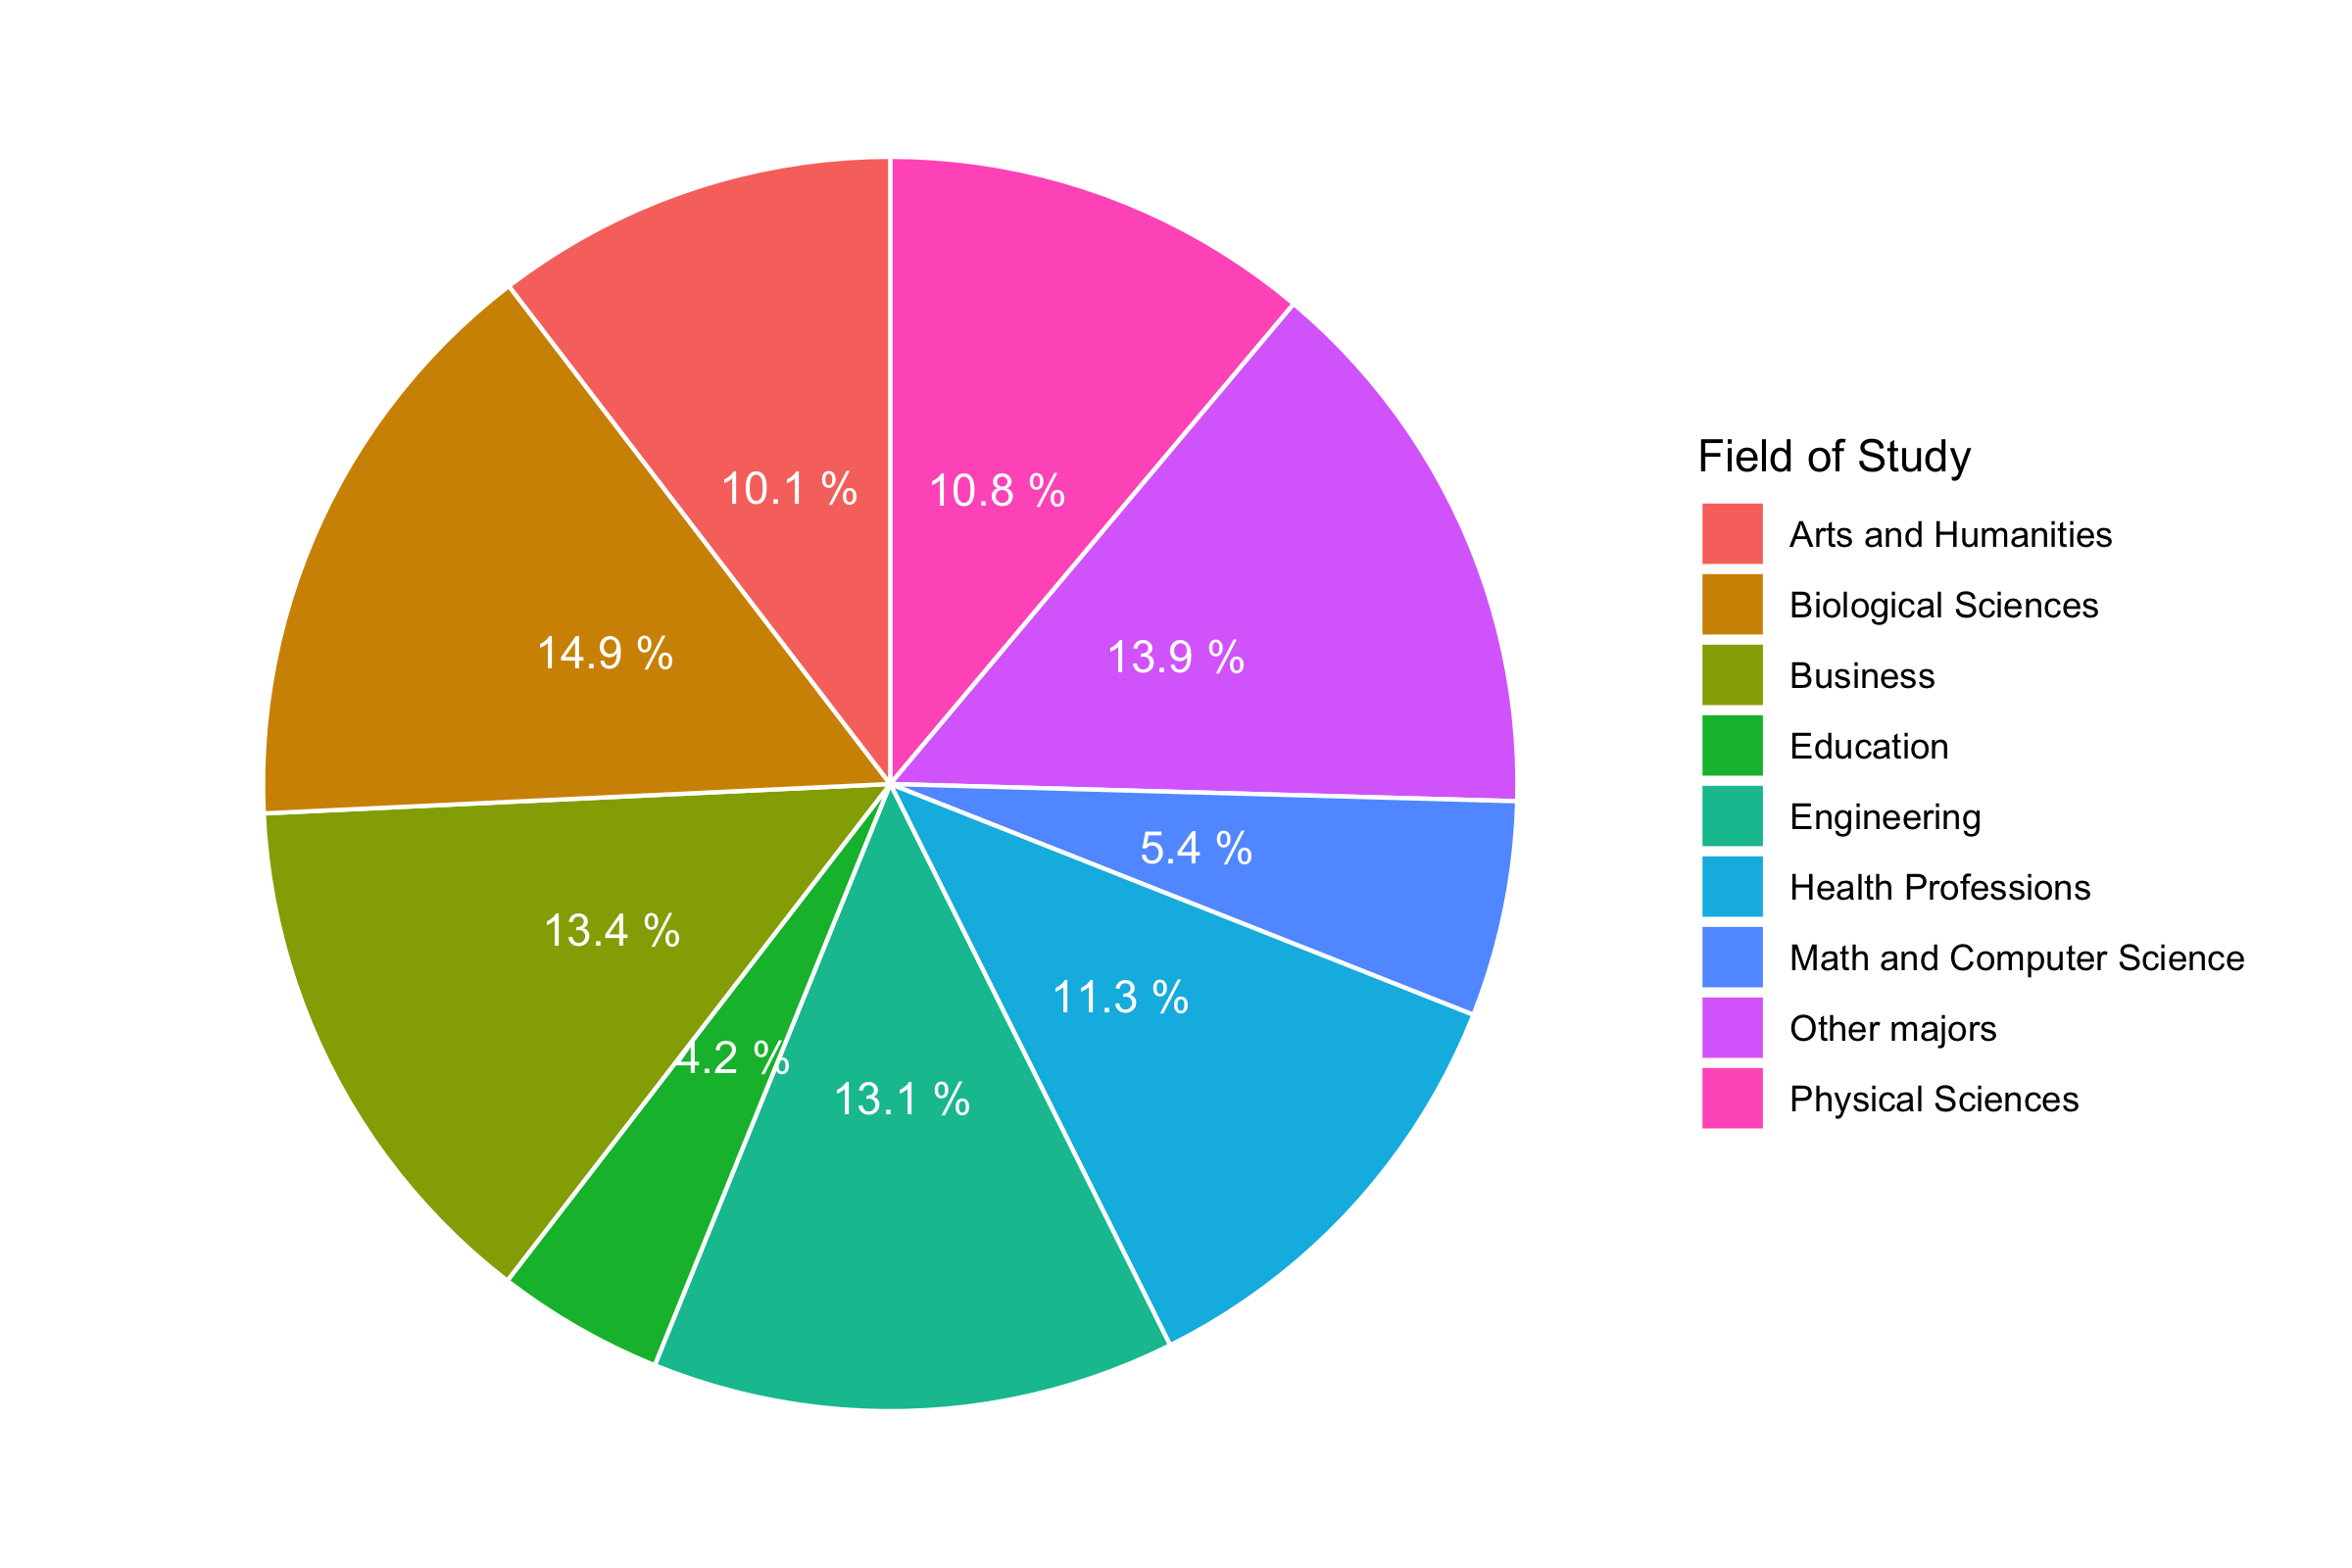
\includegraphics[width= \linewidth]{pie.png}
\end{frame}

\begin{frame}{Bar Chart}
    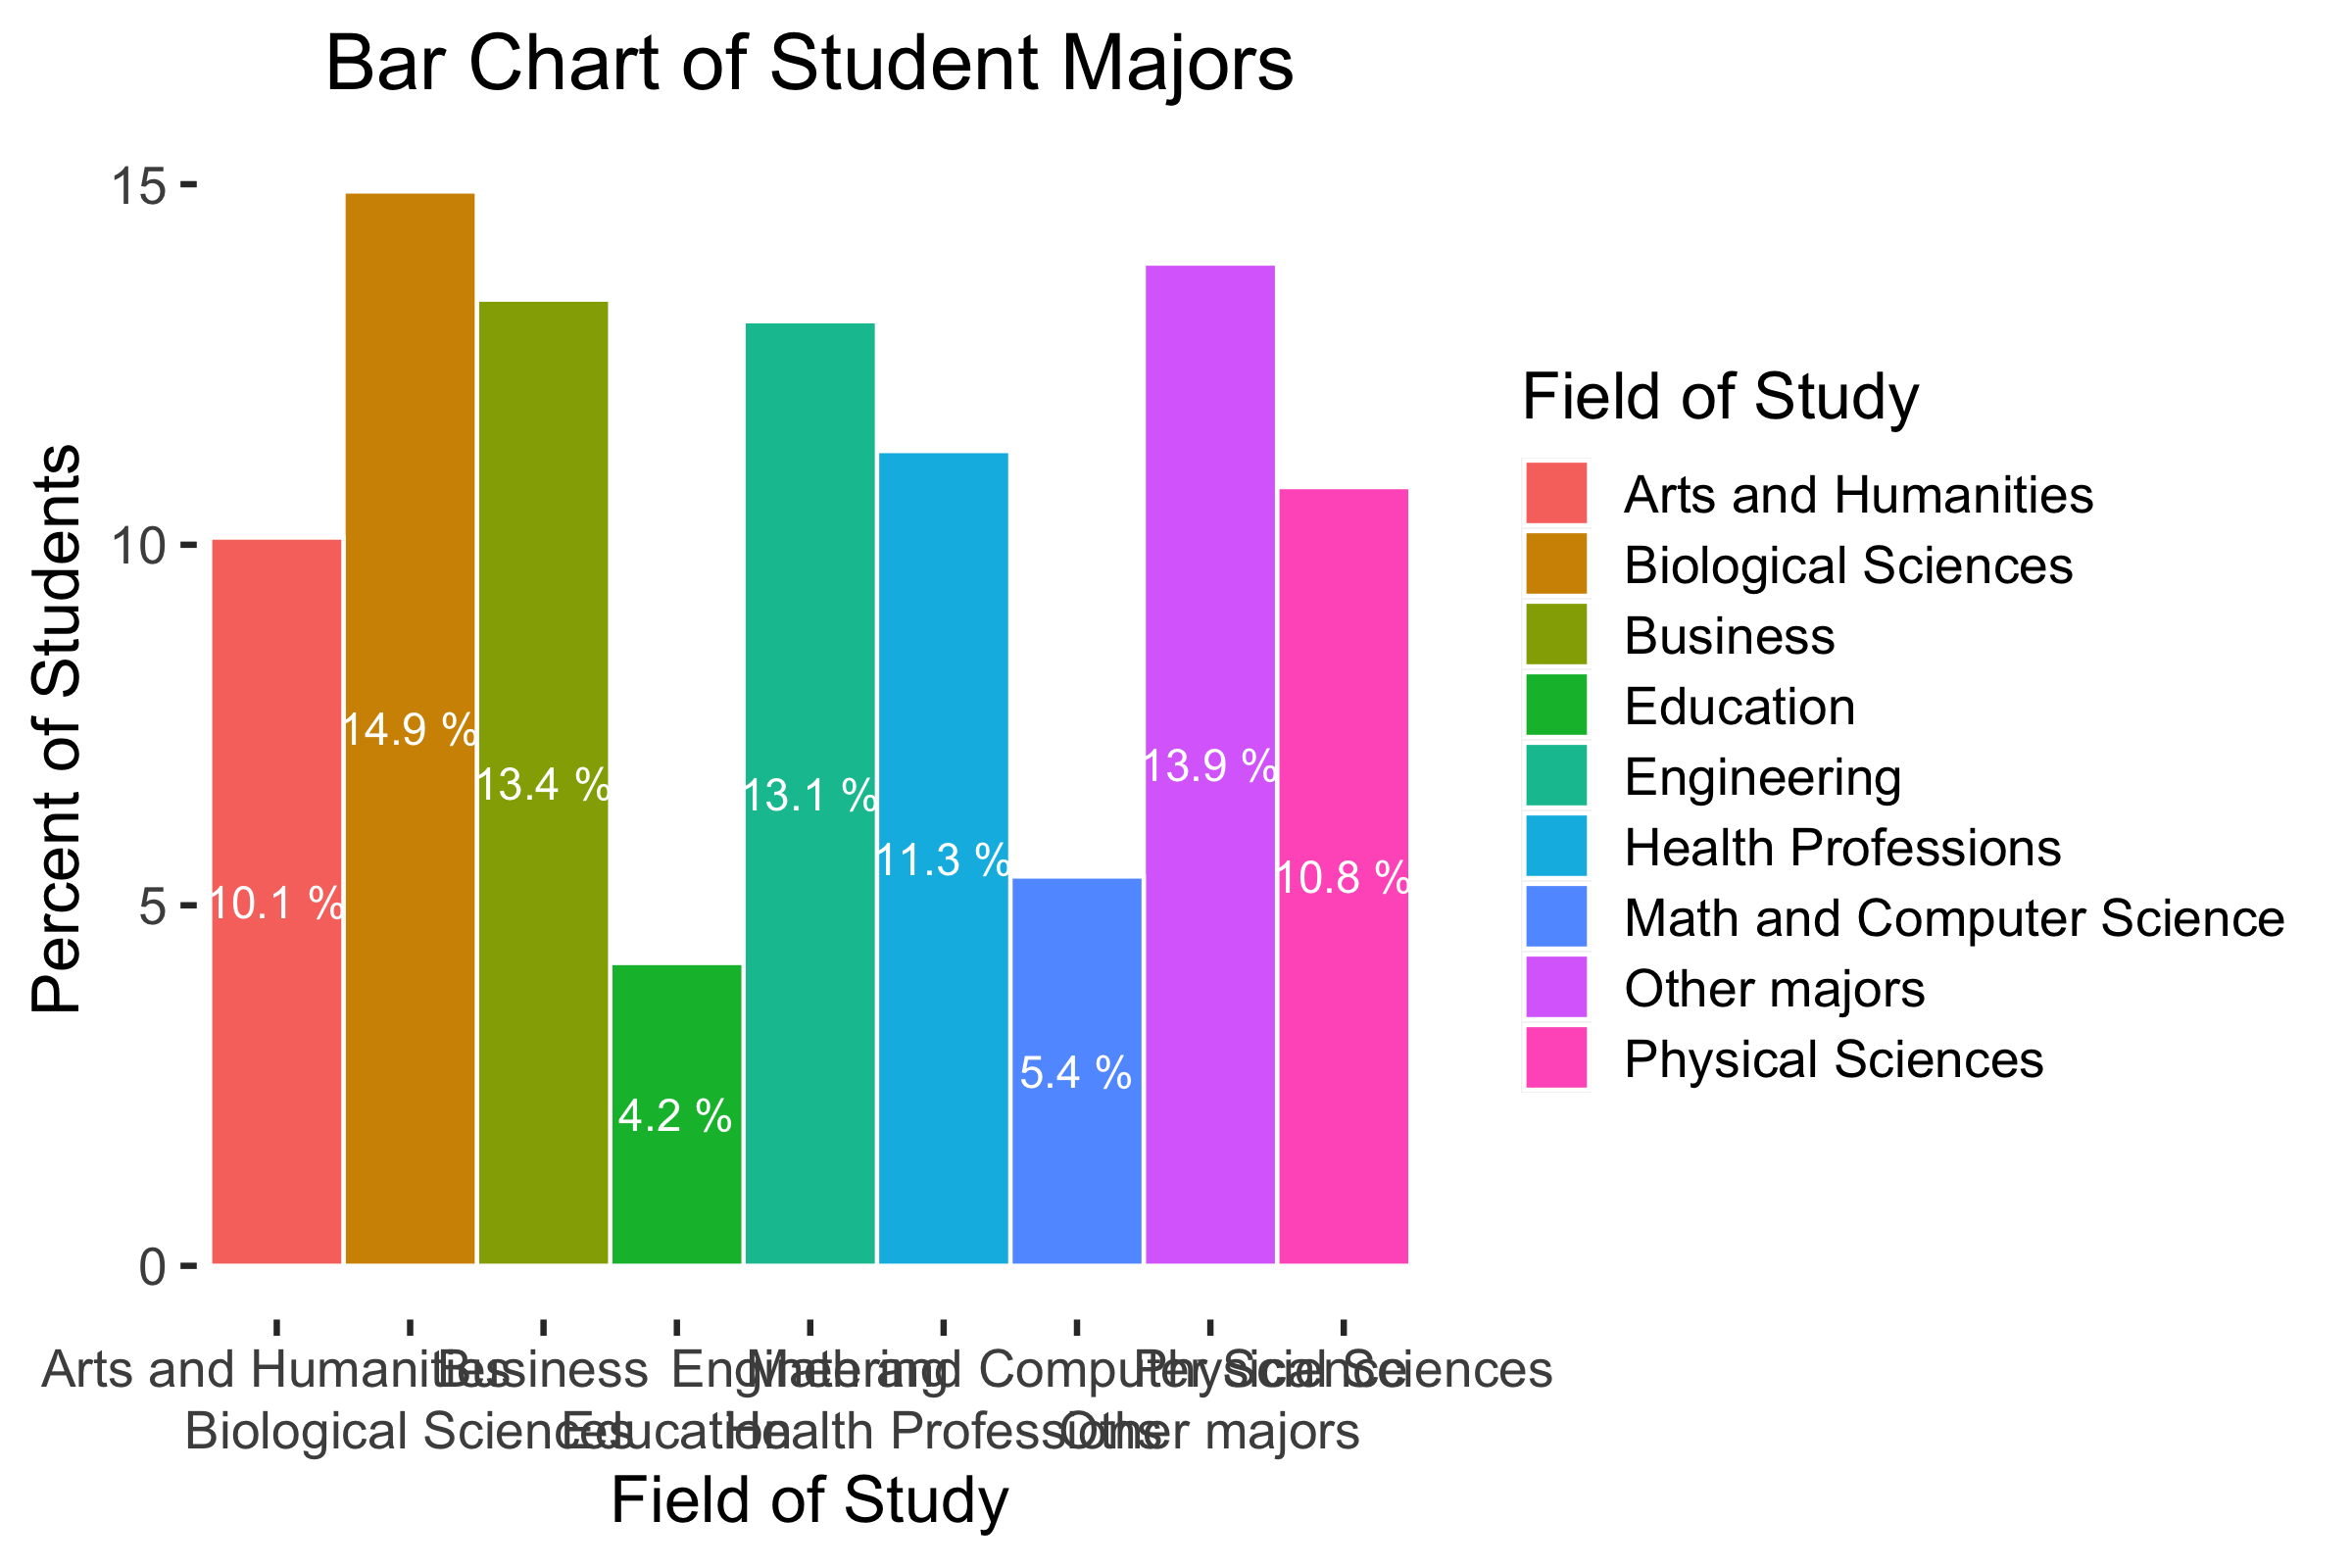
\includegraphics[width= \linewidth]{bar.png}
\end{frame}


\begin{frame}{Visualize Distributions -- Continuous Variable}
    \begin{itemize}
        \item Distribution of a quantitative variable tells us what values the variable takes on and how often it takes on those values
        \item Often visualize distributions of continuous variables using \alert{histograms}, \alert{stemplots}, or \alert{time plots} if variable is measured over time
    \end{itemize}
\end{frame}

\begin{frame}{Histogram}
    \begin{itemize}
        \item A \alert{histogram} shows the distribution of a continuous variable by using bars whose height represents number of individuals who take on a value within a particular interval (bin)
        \begin{itemize}
            \item Appropriate for variables that take on many different values or have large number of observations
        %\item To make a histogram:
        %\begin{enumerate}
        %\item Divide the possible values into intervals (bins) of equal widths
        %\item Count how many observations fall into each interval (bin)
        %\item For each interval, draw a bar whose height is equivalent to the number (or percent) of observations in each interval
        %\end{enumerate}
        \end{itemize}
    \end{itemize}
\end{frame}

\begin{frame}{Histogram Example}
    \begin{tabular}{l|r}
        \hline
        \textbf{State} & \textbf{2017-2018 Graduation Rate}\\
        \hline
        Alabama & 90.0\\
        \hline
        Alaska & 78.5\\
        \hline
        Arizona & 78.7\\
        \hline
        Arkansas & 89.2\\
        \hline
        California & 83.0\\
        \hline
        Colorado & 80.8\\
        \hline
        Connecticut & 88.4\\
        \hline
        Delaware & 86.9\\
        \hline
        District of Columbia & 68.5\\
        \hline
        Florida & 86.3\\
        \hline 
        \vdots & \vdots \\
        \hline
        Wyoming & 81.7\\
        \hline
    \end{tabular}
    
\end{frame}


\begin{frame}{Graduation Rates}
    \begin{center}
    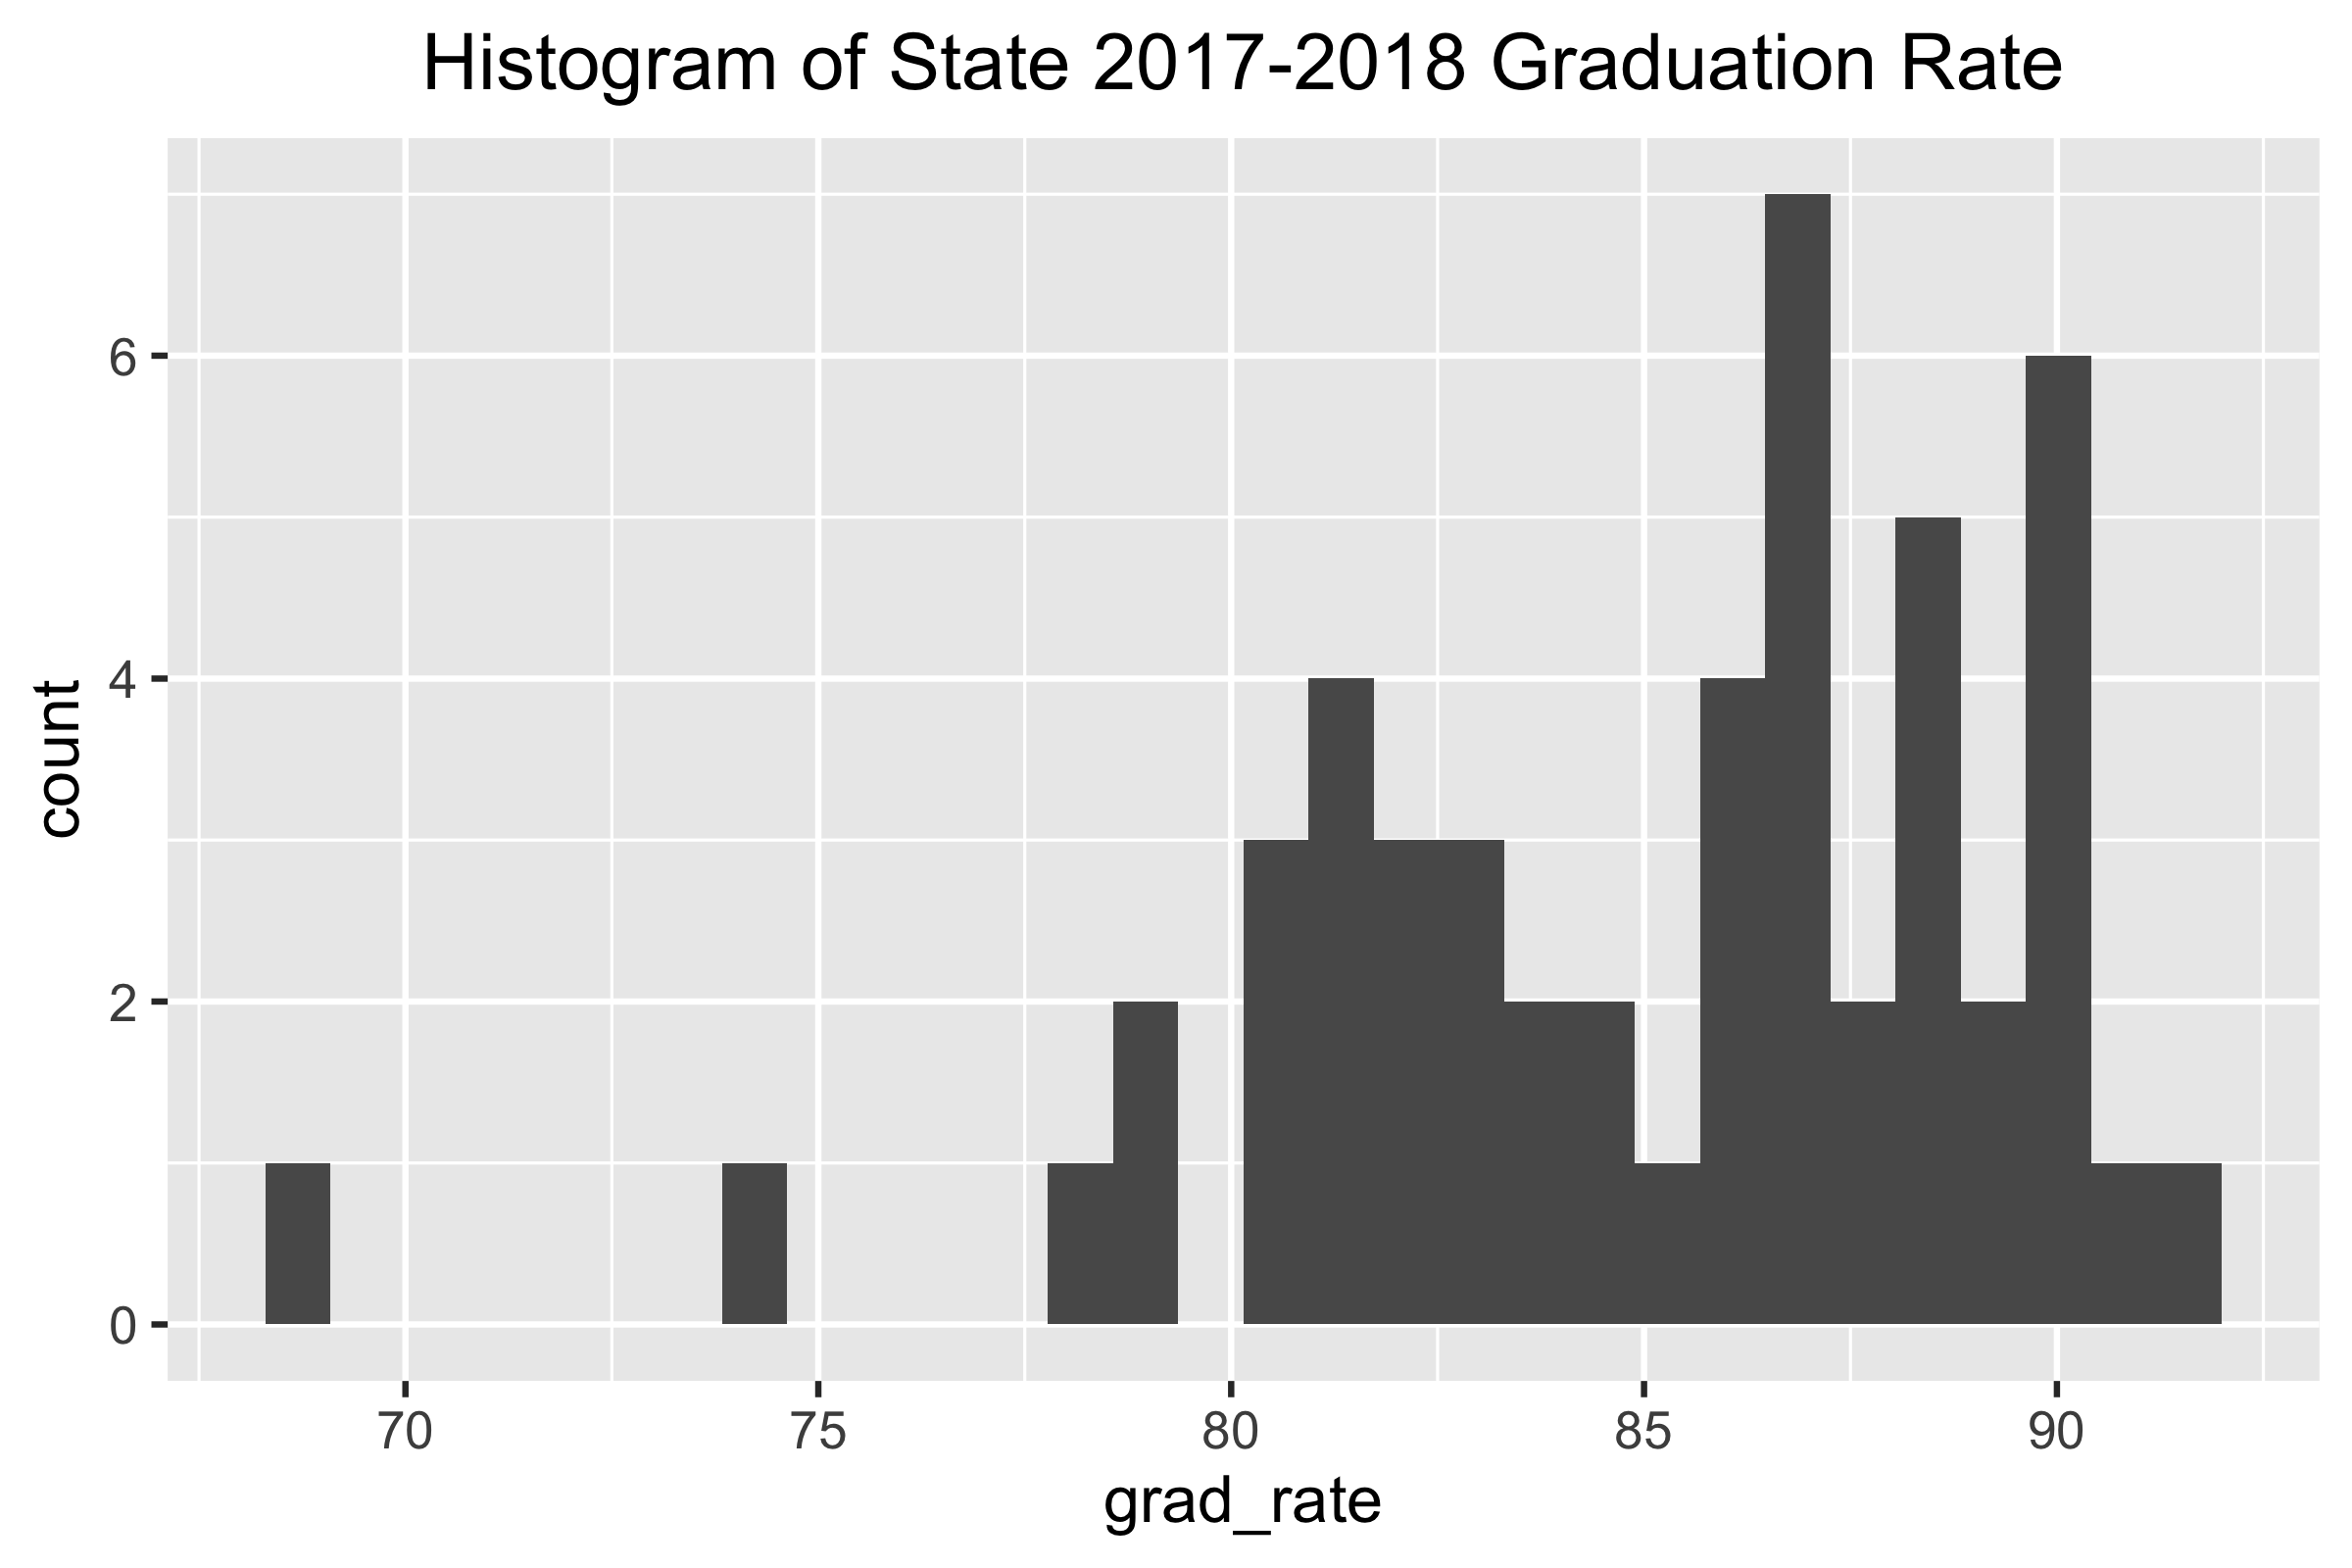
\includegraphics[width= \linewidth]{hist.png}
    {\footnotesize Data from National Center for Education Studies}
    \end{center}
\end{frame}

\begin{frame}{Interpreting Histogram}
    \begin{itemize}
        \item How to interpret histograms:
        \begin{itemize}
            \item Look for overall pattern and striking deviations from that pattern
            \begin{itemize}
                \item An important kind of deviation is an outlier, an individual that falls outside the overall pattern
            \end{itemize}
            \item Describe the pattern by its shape, center, and variability (or spread)
        \end{itemize}
    \end{itemize}
\end{frame}

\begin{frame}{Shapes of Distributions}
    We describe the shape of the distribution as
    \begin{itemize}
        \item \alert{symmetric}: the right and left sides of the graph are approximately mirror images of each other
        \item \alert{right-skewed}: the right side of the graph (containing the half of the observations with larger values) is much longer than the left side
        \item \alert{left-skewed}: the left side of the graph is much longer than the right side 
    \end{itemize}
\end{frame}

\begin{frame}{Skewness Examples}
    \begin{center}
        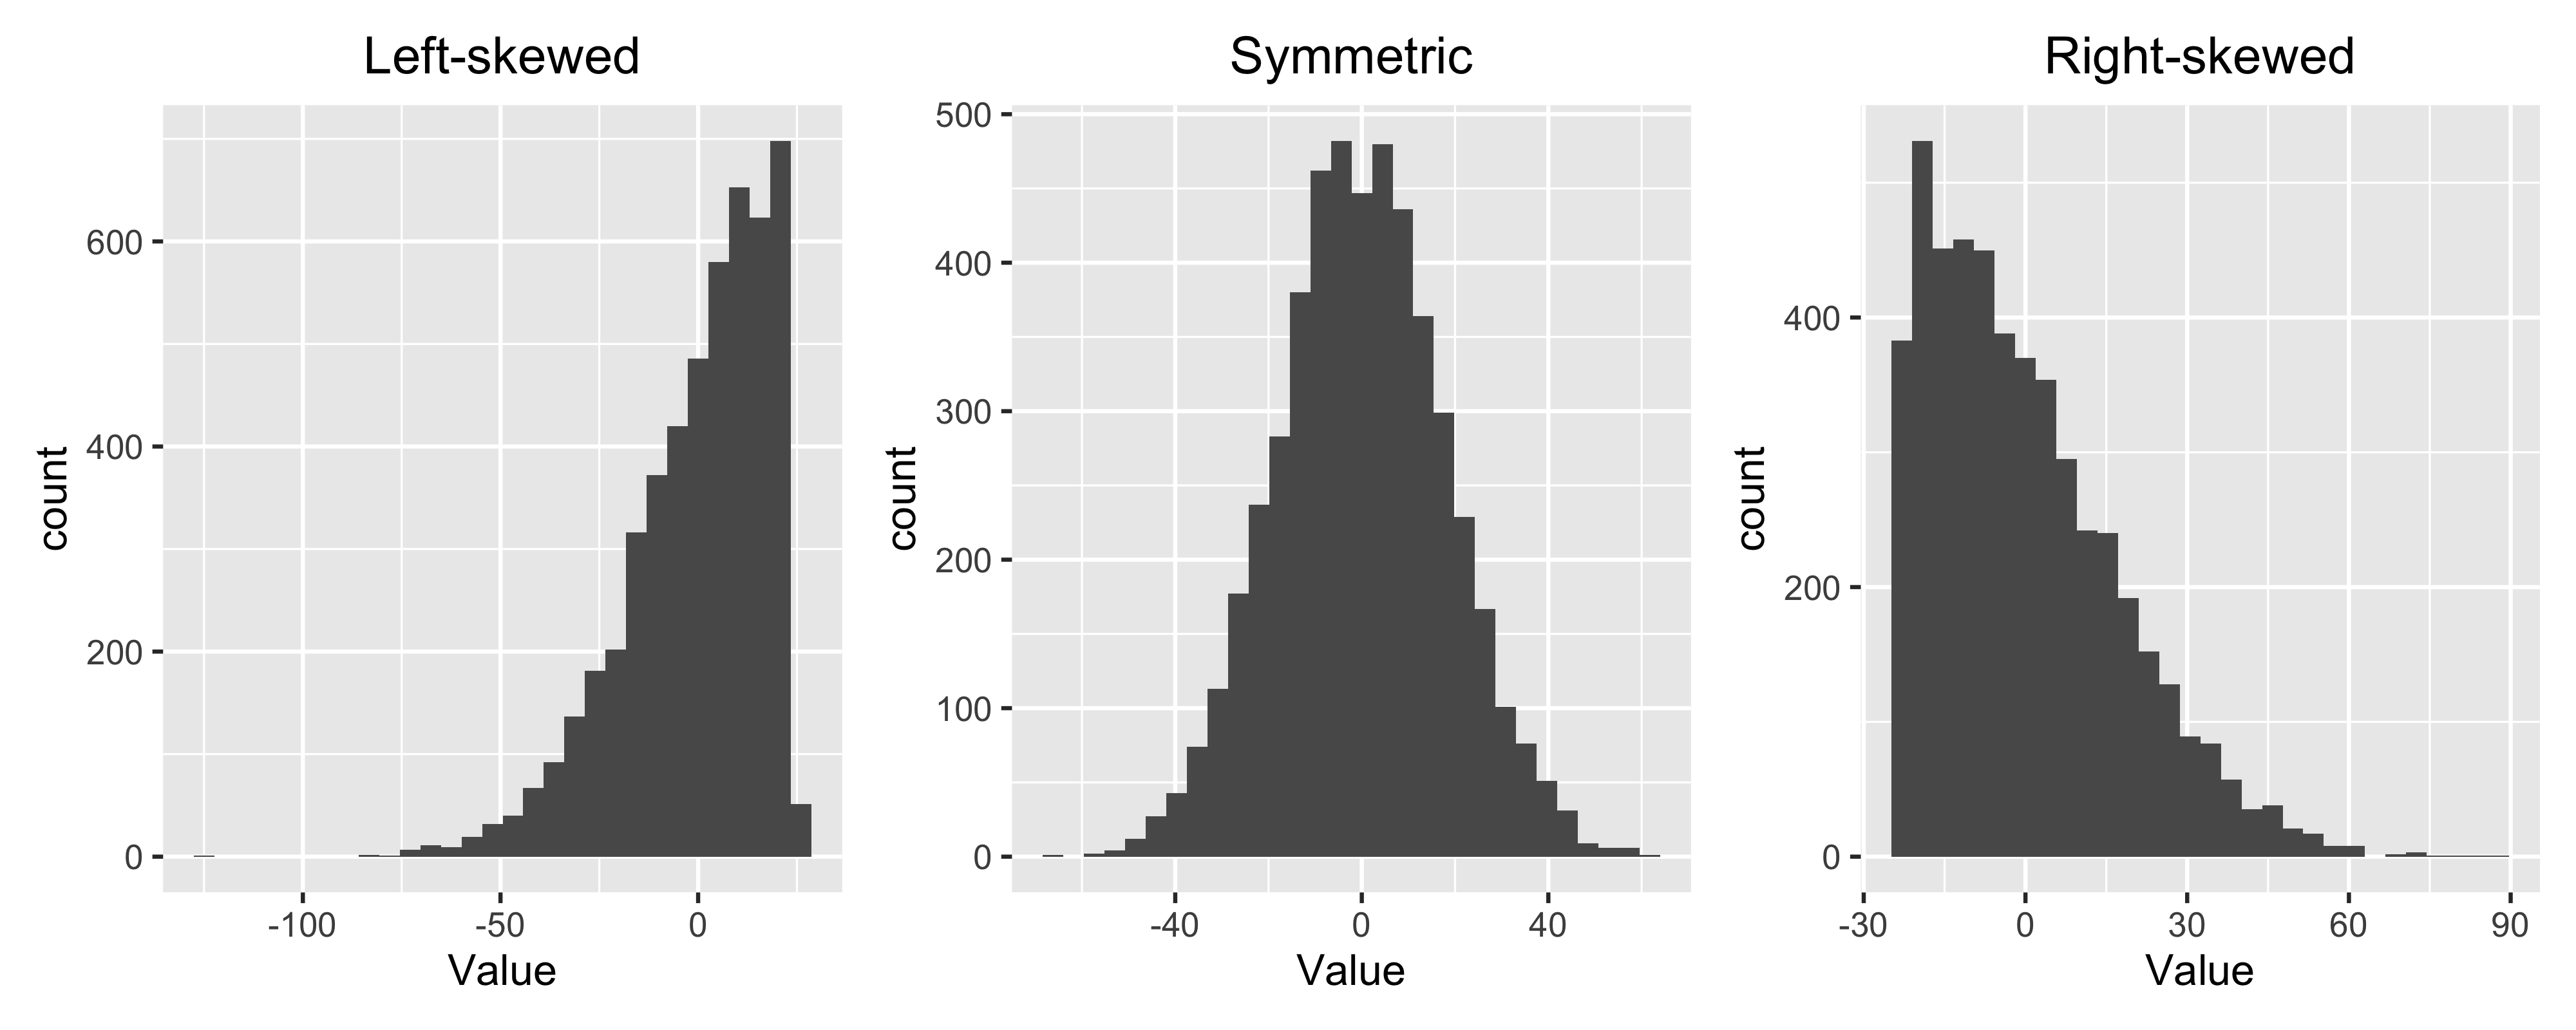
\includegraphics[width= \linewidth]{skew_plots.png}
    \end{center}
\end{frame}


\begin{frame}{Clicker Question}
    \begin{center}
        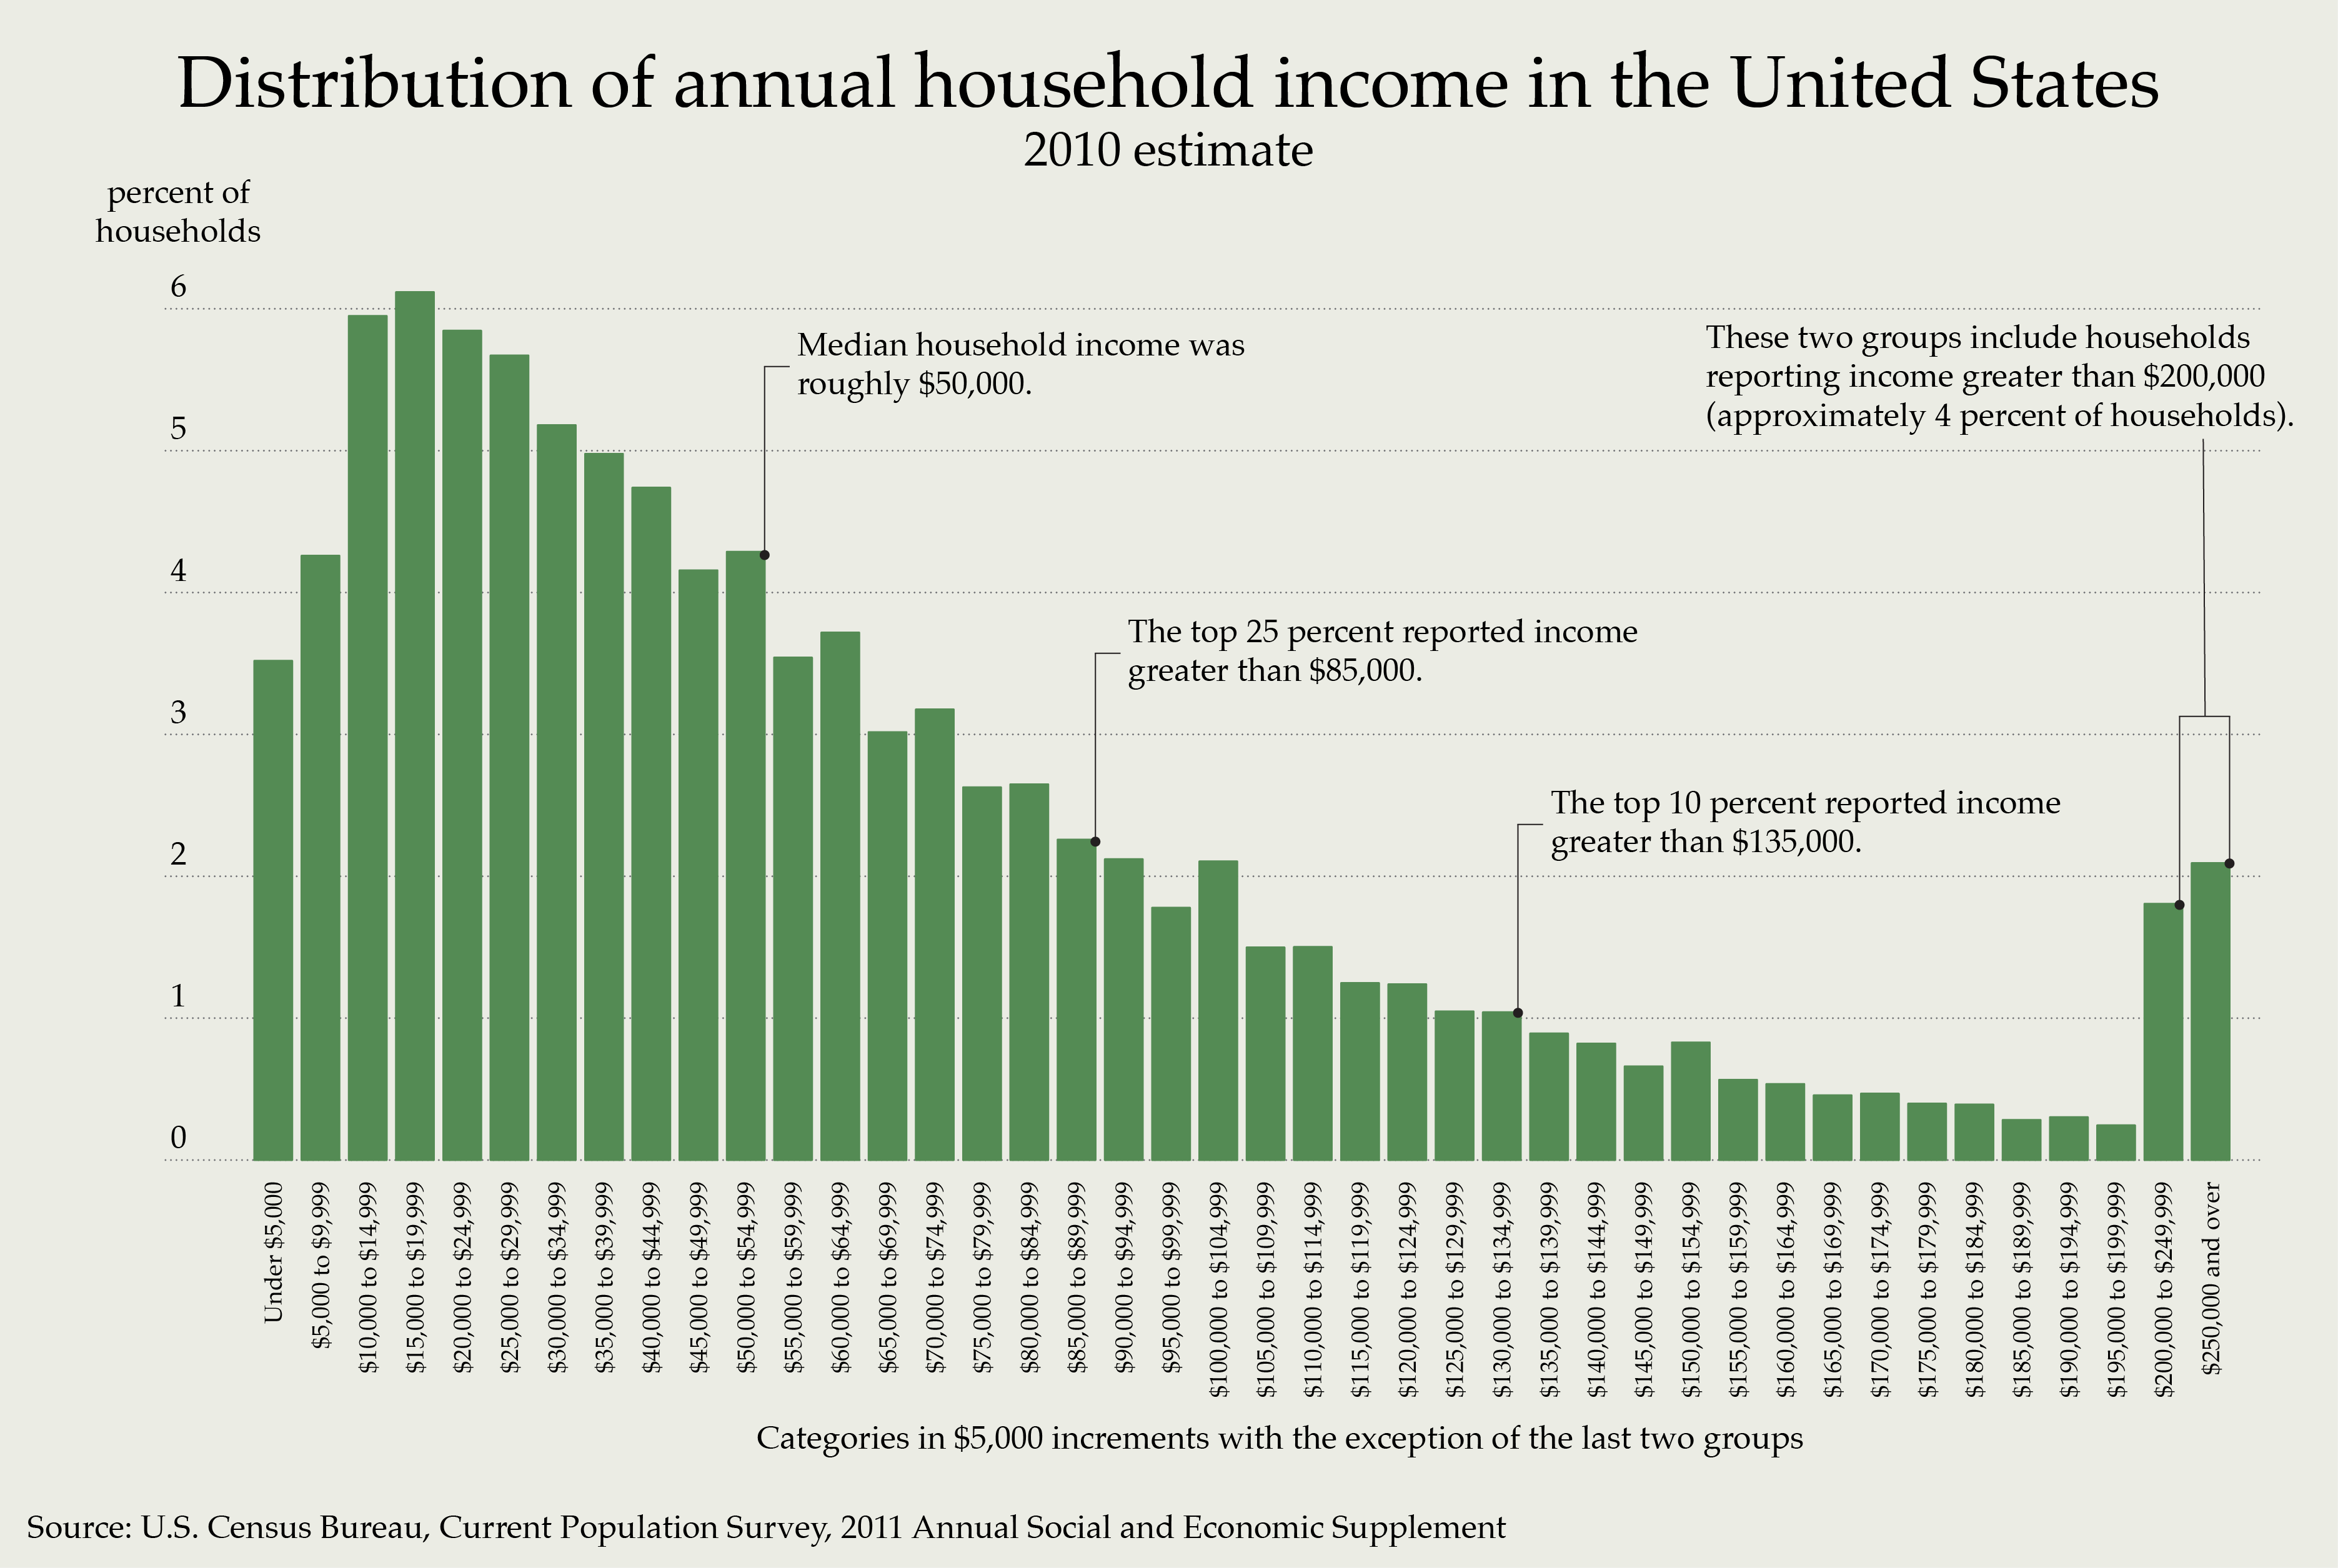
\includegraphics[width= 0.9\linewidth]{household_income.png}
    \end{center}

    (a) symmetric (b) right-skewed (c) left-skewed
\end{frame}

\begin{frame}{Clicker Question}
    For which of the following variables would you need to use a histogram instead of a bar graph?

    \begin{enumerate}[label=(\alph*)]
        \item month of birth
        \item distance from nearest metropolitan area
        \item employment status
        \item none of the above
    \end{enumerate}
\end{frame}

\begin{frame}{Time Plots}
    \begin{itemize}
        \item \alert{Time series} is a connected line plotting the value of the variable over time
        \item Shows behavior over time
        \item Time is always on the horizontal axis, variable being measured on vertical axis
        \item Connecting the data points by lines emphasizes trends
        \item Look for patterns, trends, deviations from trends
        \begin{itemize}
            \item Also want to look for seasonal variation
        \end{itemize}
    \end{itemize}
 
\end{frame}
    
\begin{frame}{Time Series Plots}
    \begin{center}
        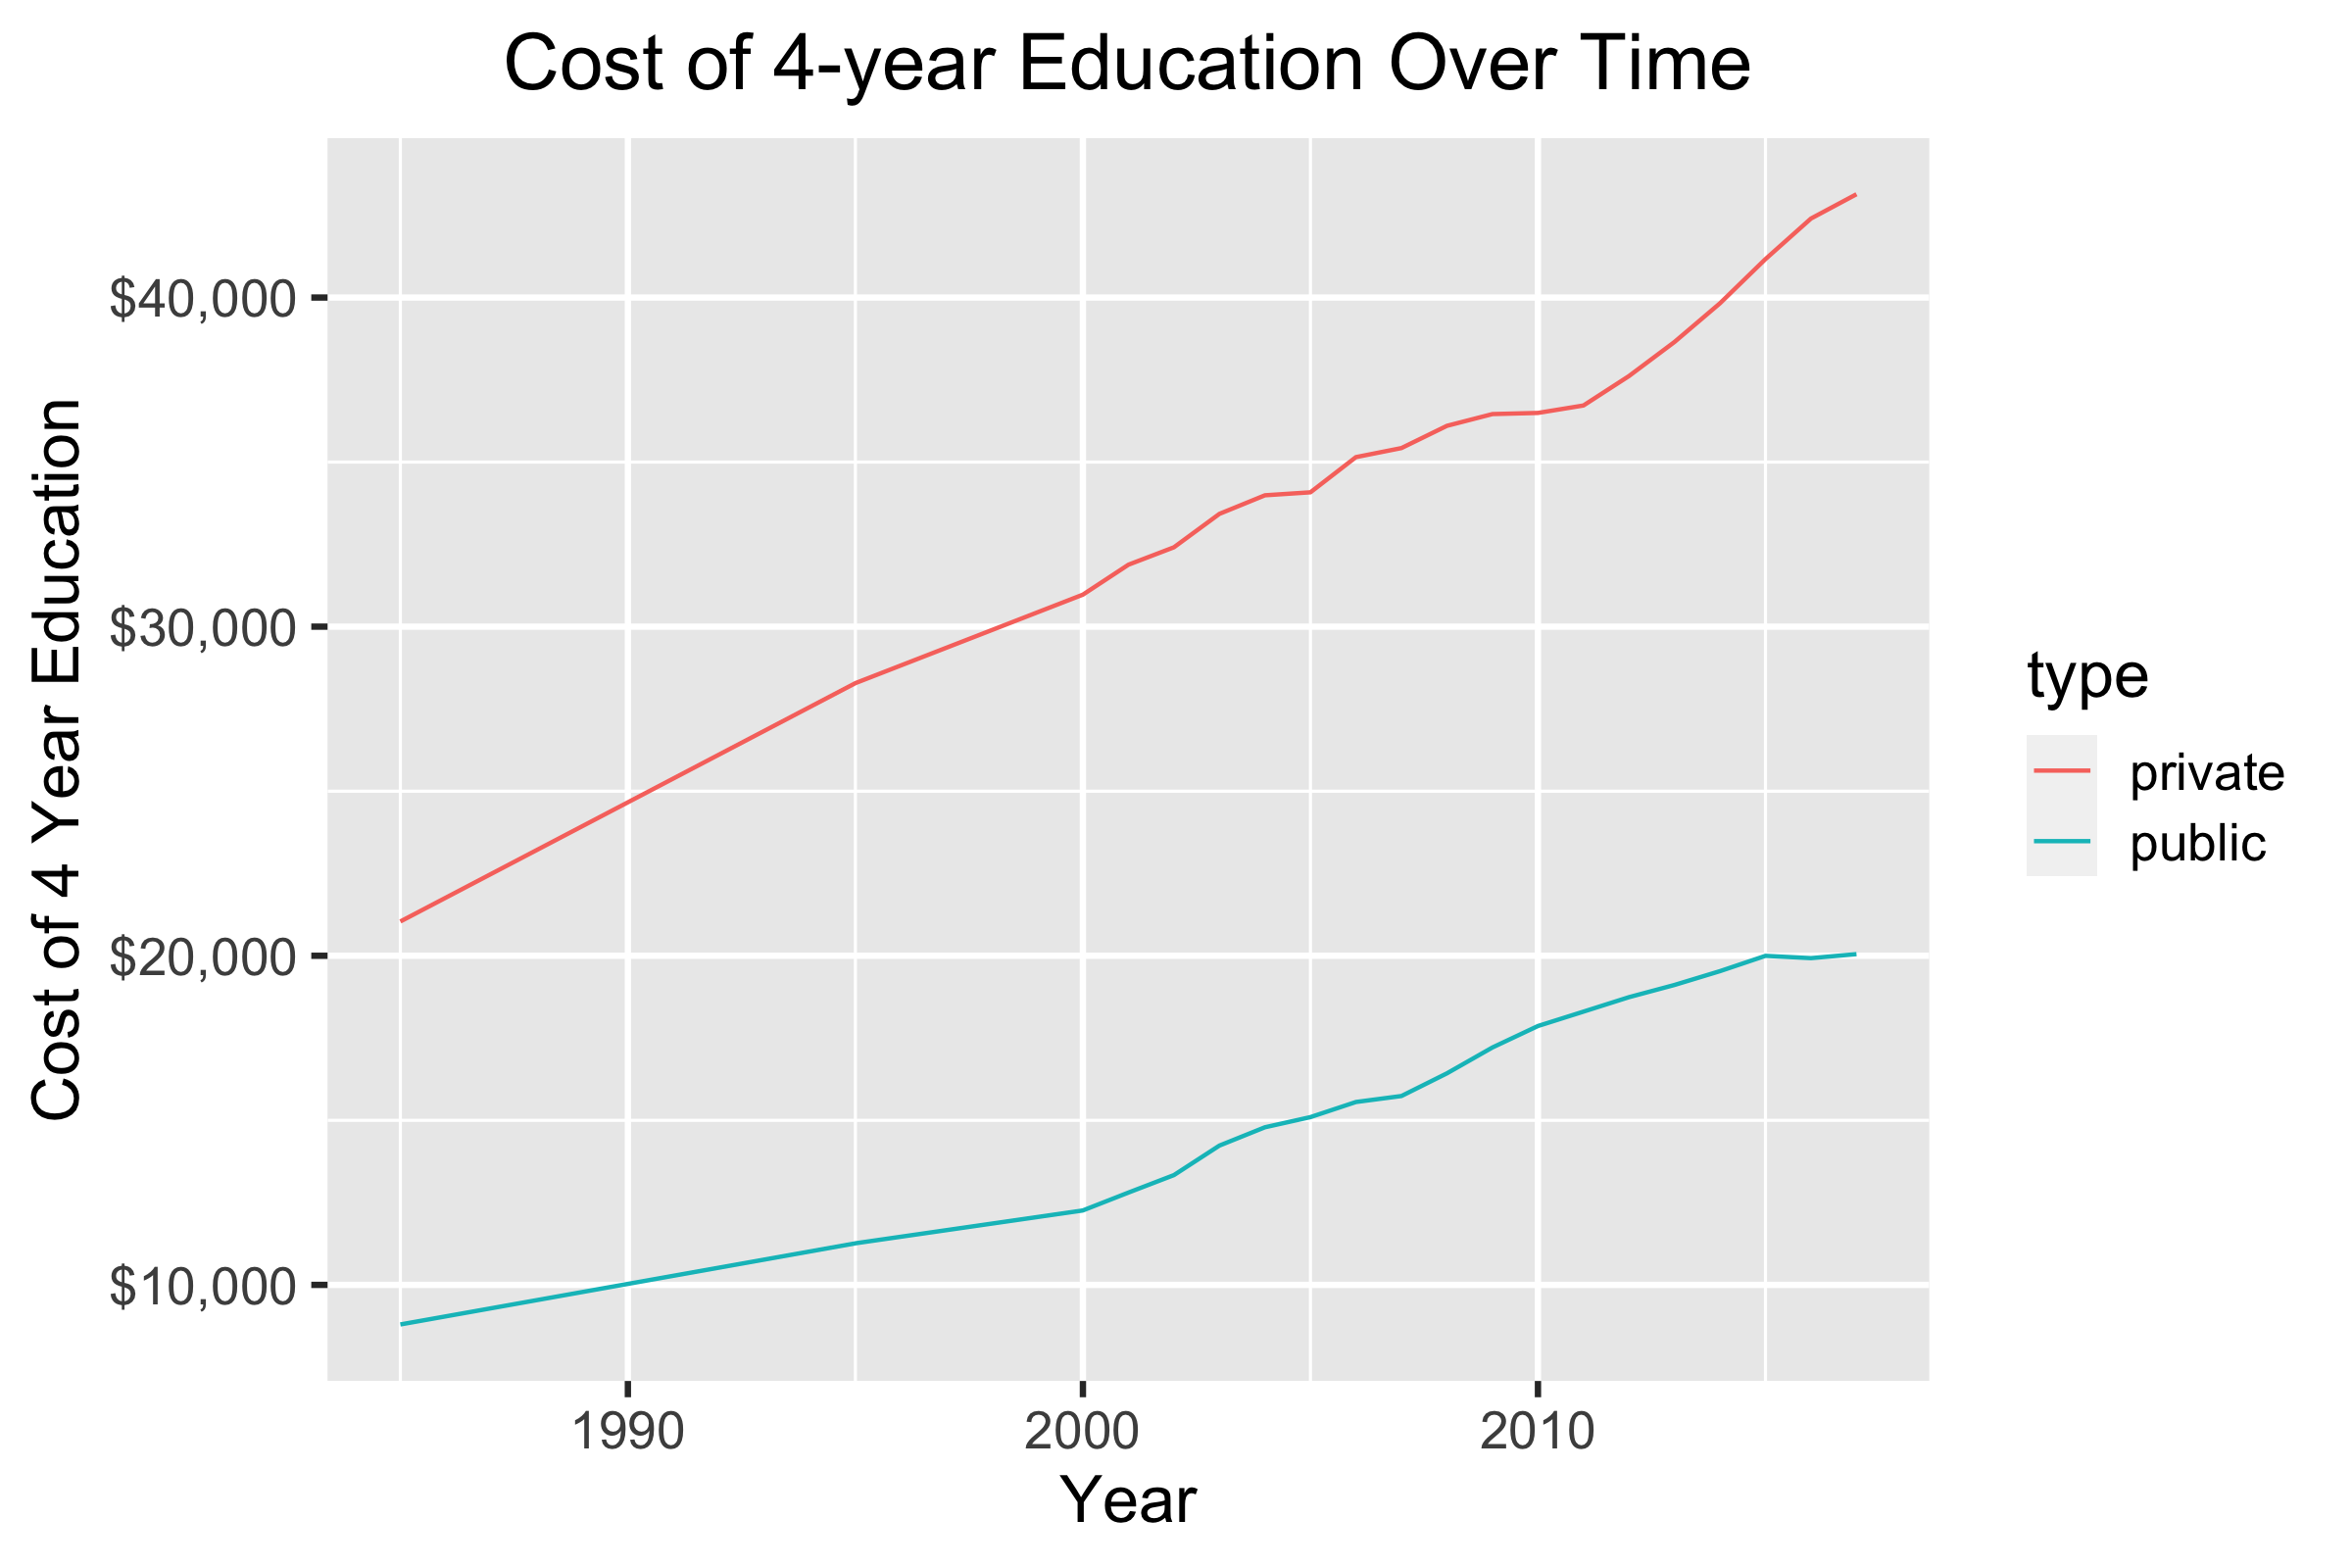
\includegraphics[width= \linewidth]{timeseries.png}
    \end{center}
\end{frame}

\begin{frame}{Clicker Question}
    Employees at a large company are surveyed about their health insurance status. Employees are coded as "1" if health insurance is obtained through the company's benefit program, "1" if health insurance is obtained from another source (such as through a spouse's employment benefit program), or "0" if the employee does not have health insurance. This variable is:

    \begin{enumerate}[label=(\alph*)]
        \item quantitative
        \item categorical
        \item both
        \item neither
    \end{enumerate}
\end{frame}










\end{document}
